\documentclass[conference]{IEEEtran}
\IEEEoverridecommandlockouts
% The preceding line is only needed to identify funding in the first footnote. If that is unneeded, please comment it out.
\usepackage{cite}
\usepackage{amsmath,amssymb,amsfonts}
\usepackage{algorithmic}
\usepackage[pdftex]{graphicx}
\usepackage{textcomp}
\usepackage{todonotes}
\usepackage{glossaries} % Acronyms
\def\BibTeX{{\rm B\kern-.05em{\sc i\kern-.025em b}\kern-.08em
    T\kern-.1667em\lower.7ex\hbox{E}\kern-.125emX}}

\graphicspath{{Figures/}}
\DeclareGraphicsExtensions{.pdf,.jpeg,.png}


%\usepackage[shortlabels]{enumerate}
\usepackage[inline]{enumitem}
%\usepackage{mdwlist}
%!TEX root = main.tex

%%%%%%%%%%%%%%%%%%%%%%%%
%%%%%%% ACRONYMS %%%%%%%
%%%%%%%%%%%%%%%%%%%%%%%%
\newacronym{ml}{ML}{Machine Learning}
\newacronym{pe}{PE}{Portable Executable}
\newacronym{dll}{DLL}{Dynamic-link Library}
\newacronym{nsrl}{NSRL}{National Software Reference Library}
\newacronym{roc}{ROC}{Receiver Operating Characteristic}
\newacronym{auroc}{AUROC}{Area Under the Receiver Operating Characteristic}
\newacronym{dr}{DR}{Detection Rate}
\newacronym{fpr}{FPR}{False Postive Rate}
\newacronym{tts}{TTS}{The Top Set}
\newacronym{tgs}{TGS}{The Good Set}
\newacronym{tpr}{TPR}{True Positive Rate}
\newacronym{tbs}{TBS}{The Bad Set}
\newacronym{lr}{LR}{Logistic Regression}

\newcommand\ie{\emph{i.e.}}
\newcommand\eg{\emph{e.g.}}

\newcommand\say[1]{``#1''}
% \newcommand\textsubscript[1]{$_\mathrm{#1}$}

\newcommand\miss[1]{\textcolor{red{#1}}}
\newcommand\dups{{dups}}
\newcommand\acc{acc}
\newcommand\mal{\mathrm{Malware}}
\newcommand\good{\mathrm{Goodware}}

\newcommand\CC{\mathcal{C}}
\newcommand\FF{\mathcal{F}}
\newcommand\LR{\mathcal{LR}}
\newcommand\DD{\mathcal{C}}
\newcommand\Cdups{\mathcal{C}_\dups}
\newcommand\II{\mathcal{I}}
\newcommand\Pf{\mathcal{P}_{f}}
\newcommand\Pl{\mathcal{P}_{l}}
\newcommand\RR{\mathcal{R}}
\renewcommand\SS{\mathcal{S}}
\newcommand\VV{\mathcal{V}}
\newcommand\VVdups{\mathcal{V}^{\dups}}
\newcommand\VVd{\mathcal{V}^{\CC}}
\newcommand\VVstar{\mathcal{V}^*}
\newcommand\DS{\mathcal{S}}

\newcommand\tp{\textrm{TP}}
\newcommand\tn{\textrm{TN}}
\newcommand\fp{\textrm{FP}}
\newcommand\fn{\textrm{FN}}
\newcommand\dr{\textrm{DR}}
\newcommand\tpr{\textrm{TPR}}
\newcommand\tnr{\textrm{TNR}}
\newcommand\fpr{\textrm{FPR}}
\newcommand\fnr{\textrm{FNR}}

\newcommand\Madups{\mathcal{M}_{\acc}^{\dups}}
\newcommand\Mad{\mathcal{M}_{\acc}^{\CC}}
\newcommand\real{\mathrm{real}}
\newcommand\loose{\mathrm{loose}}
\newcommand\strict{\mathrm{strict}}
\newcommand\Mreal{\mathcal{M}_{\real}}
\newcommand\Mrealv{\mathcal{M}_{\real}^{\VVstar}}
\newcommand\Mloose{\mathcal{M}_{\loose}}
\newcommand\Mloosev{\mathcal{M}_{\loose}^{\VVstar}}
\newcommand\Mstrict{\mathcal{M}_{\strict}}
\newcommand\Mstrictv{\mathcal{M}_{\strict}^{\VVstar}}

\newcommand\NSRL{\mathrm{NSRL}}
\newcommand\VS{\mathrm{VS}}
\newcommand\DNSRL{\CC_{\NSRL}}
\newcommand\DVS{\CC_{\VS}}	

\begin{document}


% \title{Finding the Truth: Basis for Defining ground truth and its impact in the performance of Malware Classifiers}
\title{Malware Detection via Machine Learning}

%\author{\IEEEauthorblockN{Jo\~{a}o Godinho}
%\IEEEauthorblockA{\textit{Instituto Superior T\'{e}cnico - ULisboa} \\
%\textit{name of organization (of Aff.)}\\
%City, Country \\
%email address}
%\and
%\IEEEauthorblockN{2\textsuperscript{nd} Given Name Surname}
%\IEEEauthorblockA{\textit{dept. name of organization (of Aff.)} \\
%\textit{name of organization (of Aff.)}\\
%City, Country \\
%email address}
%\and
%\IEEEauthorblockN{3\textsuperscript{rd} Given Name Surname}
%\IEEEauthorblockA{\textit{dept. name of organization (of Aff.)} \\
%\textit{name of organization (of Aff.)}\\
%City, Country \\
%email address}
%\and
%\IEEEauthorblockN{4\textsuperscript{th} Given Name Surname}
%\IEEEauthorblockA{\textit{dept. name of organization (of Aff.)} \\
%\textit{name of organization (of Aff.)}\\
%City, Country \\
%email address}
%\and
%\IEEEauthorblockN{5\textsuperscript{th} Given Name Surname}
%\IEEEauthorblockA{\textit{dept. name of organization (of Aff.)} \\
%\textit{name of organization (of Aff.)}\\
%City, Country \\
%email address}
%\and
%\IEEEauthorblockN{6\textsuperscript{th} Given Name Surname}
%\IEEEauthorblockA{\textit{dept. name of organization (of Aff.)} \\
%\textit{name of organization (of Aff.)}\\
%City, Country \\
%email address}
%}

\maketitle

\begin{abstract}
%!TEX root = main.tex

The use of supervised learning techniques for malware detection has been used increasingly to aid classical classification methods. 
In this work we aim at developing a malware detection model, analyzing the impact of the reliability of the training dataset on the final result of the classifier, and metrics to define the \emph{ground-truth}.
For this, we propose three datasets' scenarios whose content range from unambiguous malware and goodware samples to more ambiguous and real ones.
We analyze each scenario in laboratory conditions, where standard cross-validation methodologies are applied, discarding the importance of \emph{time} in malware detection, and also in real-world conditions, where temporal-based dependencies are proposed and applied.
Furthermore, we modify our original model to both enrich the extractable information, by implementing a multi layer model, and to improve the final results, by using dynamic information about the samples.
We then use our temporal-based methodologies to reduce the size of the training dataset without compromising optimal results, concluding that there exists an ideal number of necessary training folds, temporally consistent with the validation fold, that maximizes the overall score.
\end{abstract}

\begin{IEEEkeywords}
Security,
Malware Detection,
Machine Learning,
Temporal Consistency,
Ground Truth
\end{IEEEkeywords}

%!TEX root = main.tex


\section{Introduction}\label{sec:intro}

The number of reported security breaches due to \emph{virus}, \emph{worms}, \emph{trojans}, etc, has been growing considerably in recent years~\cite{av-test:report} with reports of infections due to \emph{malware}  making the headlines, now more than ever.
Almost every week one such security vulnerability is reported which may be seen as a failure by the security community on the control and detection of malicious content. 

The very first challenge that we face is the definition of \emph{malware}.
Malware is considered to be \say{a program with malicious intent}~\cite{christodorescu:semantics} which in itself is a dubious definition. 
Not only the same programs are classified differently as \emph{malware} and \emph{goodware} depending on the vendor, but also some programs fall within a gray area for which no clear classification can be deemed correct.
An example is what is called \emph{adware}, advertising-supported software, that although not performing directly malicious actions, perform arguably non-requested actions.
The non-existence of concrete metrics and properties that uniquely distinguish malware from goodware requires an extra effort in the preparation of datasets for evaluation of malware detectors.

Due to the significant number of malware attacks, and taking into consideration the increasing popularity and huge success of \gls{ml} methodologies in classification in different domains~\cite{lee2003learning,joachims2002learning,li2010object,ding2001multi}, it is only natural to see these techniques applied to complement classical methodologies for malicious-content detection~\cite{arp2014drebin,christodorescu:semantics,kolosnjaji2016deep,kolter:learning,miller:rev_int,nissim:al_pdf,perdisci:behavior,rieck:dynamic,santos2013opcode,schultz:data_mining,schwenk2012autonomous,vsrndic2013detection,deo2016prescience,gandotra2014malware,jordaney2017transcend,rossow:practices}, in particular, supervised learning techniques.
However, several issues have arised regarding the usage of these ML techniques in the scope of malware analysis~\cite{deo2016prescience,gandotra2014malware,jordaney2017transcend,rossow:practices}.

On the sometimes ambiguous scenario that is the task of distinguishing malware from goodware, some of these results largely depend on the datasets used for evaluation, often not representing the real-world. 
In this paper we address this pertinent questions and make a comparative analysis of a supervised learning approach in three different scenarios (depicted in Figure~\ref{fig:scenarios}): a \emph{strict scenario} where only very well-characterized samples are considered, a \emph{loose scenario} where a wider set of still well-studied samples is considered, and finally a \emph{realistic scenario} where we get closer to the reality faced by vendors of malware detection solutions.

\begin{figure}[!h]
	\centering
	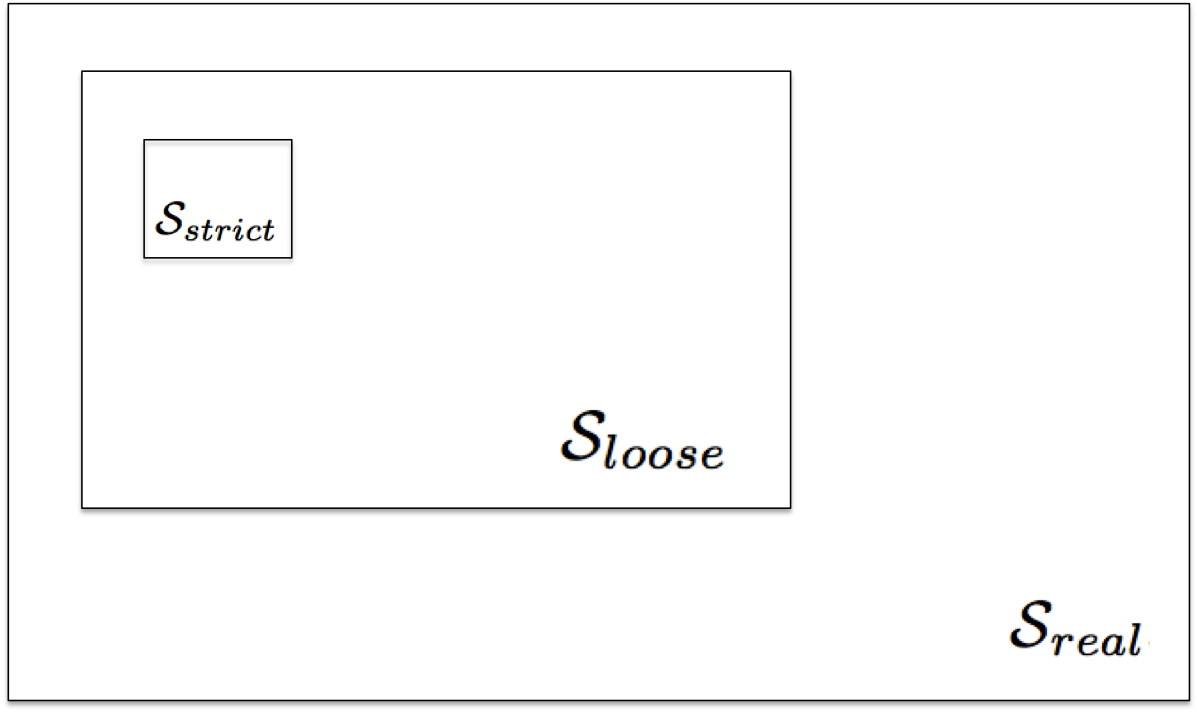
\includegraphics[width=2.5in]{dataset_sizes}
	\caption{Representation of our $\mathcal{S}_{strict}$, $\mathcal{S}_{loose}$ and $\mathcal{S}_{real}$ scenarios.}
	\label{fig:scenarios}
\end{figure}

Throughout this work we will perform a comparative analysis of the three above scenarios under two distinct environments:

\begin{itemize}[noitemsep]
	\item \emph{laboratory conditions} where traditional cross-validation methodologies can be applied;
	\item \emph{real-world conditions} where time is relevant and we analyze the behavior of the classifier with temporal-based methodologies.
\end{itemize}

We show that without much tweaking, and using simple features, a \gls{lr} model is able to achieve an \gls{auroc} of 0.91 when ideal laboratory conditions are met, but these results go down to an \gls{auroc} of 0.75 when we change into a real-world scenario.

With the purpose of actually evaluating the usage of \gls{ml} methodologies for malware detection as a complement to traditional malware detection techniques, we also analyze how the size of the training set can influence the performance of the classifier under the three studied scenarios.
For this, we use the aforementioned temporal-based methodologies to come up with conclusions on how large the training set need to be to ensure optimal results from the classifier.

We finish off by improving our base model to include more dynamic features, as well as providing a multi layer approach which adds the ability of classifying malware samples from different classes, in contrast with simply providing if a sample is malware or not.
These improvements boost our \gls{auroc} to 0.98 in ideal laboratory conditions and 0.95 in a real-world scenario.

As the main contributions of this paper
\begin{enumerate*}[label={\alph*)},font={\color{red!80!black}\bfseries}]
	\item we propose three different scenarios to train and validate the model which range from a more simulated scenario to a more realistic one,
	\item temporal-based methodologies to train and validate the classifier, 
	\item we study how much can we reduce the training dataset without compromising the optimal results,
	\item we improve our base model by 7\% to 27\%.

\end{enumerate*}


This paper is outlined as follows: in Section~\ref{sec:related} we present
the related work and justify how it motivated our work; in Section~\ref{sec:data} we describe and analyze the available dataset and how it was labeled; in Section~\ref{sec:feature_model} we propose a feature selection and describe the used model; Section~\ref{sec:eval_results} encloses our main contributions, describing our three scenarios and how they are to be evaluated, using regular cross-validation and our defined temporal-based methodology, together with the results of said evaluation;
in Section~\ref{sec:improvements} we provide improvements to our base model; in Section~\ref{sec:discussion} we discuss our main achievements; Section~\ref{sec:conclusion} concludes the paper and discusses avenues for further research.

%!TEX root = main.tex

\section{Related Work}\label{sec:related}

We use this section to present prior work that closely relates to the topic of our research and our areas of contribution. Specifically, detecting malicious software by training supervised models on static information, and validation methodologies that resemble real-world conditions.

Shabtai et al.\cite{shabtai:survey} provide a survey directed
at the application of \gls{ml} classifiers to detect malware from static
features. Their work concerns the design and evaluation of such systems. Our contributions are inspired by the concern of how to correctly evaluate \gls{ml} classifiers, regarding size, reliability of labeling metrics and chronological evaluation.

In the topic of methodologies that resemble real-world conditions, Srndi\'c et al.\cite{vsrndic2013detection}
train and validate their malicious PDF detector under laboratory and real-world conditions. Laboratory conditions consist on applying regular cross-validation, whereas real-world conditions validate a newer dataset with a model created from outdated data (i.e.\ older then the validation), and also validate the model when the validation set spans one week and the training is gathered in the previous 4 weeks. They show that laboratory conditions inflate the results, when compared to real-world conditions.

Miller et al.\cite{miller:rev_int} also introduce sample temporal consistency. They show the impact of performance measurement technique on a dataset containing 1.1 million samples, when using cross-validation and temporally consistent samples. As noted by others, regular cross-validation showed inflated results when compared to temporally consistent samples.

Our work enhances these methodologies by analyzing the performance variation when the distance between the training and validation set increases and decreases, as well as analysis on how reducing the size of the training without compromising the results.

Kolter et al.\cite{kolter:learning} learn to detect malicious executables in a dataset with under 4,000 samples, obtained from reliable sources, and evaluate their model under standard cross-validation and by gathering newer malware samples to validate for new and unseen samples. They show how the model provides optimal results under cross-validation, but for the unseen samples lower scores are obtained. Our work considers these results to compare how reliability affects performance.

Sebastián, M. et al.\cite{sebastian2016avclass} develop \textit{AVClass}, a tool that given a set of antivirus vendors, outputs the most likely family name. They test their tool under 10 datasets, totaling 8.9 M samples, with results showing an F1 measure up to 93.9 on labeled datasets. The tool takes as input the labels as seen in VirusTotal, tokenizes the labels, replaces known aliases and general names (e.g.\ win32, trojan, generic), ending with possible family names. These remaining names are counted and the most frequent one is given as family name. Our work takes advantage of this tool, not to label malware families, but minimal modifications, to label more general malware classes (e.g.\ trojan, virus).

Deo, A. et al.~\cite{deo2016prescience} focus over the problem of \gls{ml} models becoming antiquated over time, given how malware evolves. This problem is seen as concept drift, where the performance of a model over time diminishes, as the statistical properties of malware (i.e.\ features) change over time. They study how probabilistic predictors can help minimize the aforementioned problem, by indicating when retraining of a given model is necessary. 

Jordaney, R. et al.~\cite{jordaney2017transcend} also study the problem of concept drift in malware classification models, focusing on providing metrics, based on statistical comparison of samples, to detect when should a model be retrained. 

Both ~\cite{deo2016prescience} and ~\cite{jordaney2017transcend} are on the subject of our work, regarding the problem of concept drift, but differ on the study-case. In our work we acknowledge the concept but focus on its relative effects and how one can balance the size of needed training data vs. validation data, when maintaining a temporal consistent dataset. Whereas their work provide indicators for when should a model be retrained when the problem of concept drift becomes significant.
%!TEX root = main.tex
\color{black}

\section{Data Collection, Analysis and Labeling}\label{sec:data}

Malware classification is non-deterministic task, as several nuances make vendors disagree on what they classify as malware. Not only subtleties related to programs such as \emph{adware} or \emph{remote management consoles}, for which one can find arguments to classify them in either class, but also because some vendors are more accurate than others when classifying malware.

In order to be able to study how \emph{temporal consistency} and \emph{ground truth} influences a model trained to detect malicious and non-malicious applications, we gathered a large dataset of publicly available samples that includes both \emph{malware} and \emph{goodware} with no a priori labeling.

In this section we will provide an overview of the collected data, in particular its sources, followed by an analysis on these samples, and a discussion on the cross-checking mechanisms we used to perform the labeling. In the end of this section we will provide 3 metrics for analysis that differ in the confidence one can provide on the samples' labeling.

\subsection{Data Sources}\label{sub_sec:data_collection}

To study how \emph{temporal consistency} and \emph{ground truth} influences a model trained to detect malicious and non-malicious applications, we started by gathering a dataset of malware and goodware.
This dataset was obtained from \emph{Malwr}~\cite{tool:malwr}, an online service that runs static and dynamic analysis on user submitted files using \emph{Cuckoo Sandbox}~\cite{tool:cuckoo}.
Although Malwr accepts any kind of file, we are interested solely in \gls{pe} files, not only because Windows' systems are relevant targets of malicious applications, but also due to the fact that our initial approach will focus on static information obtained from these \gls{pe} files.

Malwr service provides the analysis of the submitted files as well as the MD5 of such files, but no labeling as whether a sample corresponds to a malicious or non-malicious application.
To perform this labeling we use the anti-virus' signatures given by \emph{VirusTotal}~\cite{tool:virustotal} at the time of analysis (incorporated in Malwr's reports), as a means of labeling the gathered reports.
VirusTotal is an online service where one can submit a suspicious file and in return obtain a list with the analysis performed by a significant number of vendors on whether the sample is clean or not. 

However, and as mentioned before, these classifications are not unanimous, and we still need to assign a labeling to each sample.
For this reason, we enrich our knowledge regarding samples' ground truth by aggregating metadata from \emph{\gls{nsrl}}~\cite{tool:nsrl} and \emph{VirusShare.com}~\cite{tool:virusshare}, specifically the samples' MD5. 
NSRL contains a collection of digital signatures of known, traceable software applications, whereas VirusShare.com is a repository of malware samples, so a sample belonging to the \gls{nsrl} set gives us a higher confidence that it is indeed goodware, whereas one belonging to VirusShare.com set gives us a higher confidence that it is malware. 

In summary, we collected reports from the \gls{pe} samples available in Malwr, and complemented it with metadata from \gls{nsrl} and VirusShare. The following subsection quantifies our \textit{corpus}, providing a better understanding of the available samples.


\subsection{Data Analysis}\label{sub_sec:data_analysis}
We collected our data from Malwr between April 16th, 2013 and October 10th, 2016.
Our data can be divided in three sets:
\begin{enumerate*}[label={\alph*)},font={\color{red!80!black}\bfseries}]
	\item a set $\RR$ of raw reports, containing 388,702 \gls{pe} samples; 
	\item a set $\CC\subseteq\RR$ of 284,880 classified reports by 38 vendors ($\mathcal{V}$) that is obtained by restricting the original set $\RR$ (that includes 97 vendors) to those reports whose vendors are present in at least 95\% of the classified samples.
\end{enumerate*}
% Our working dataset $\DD=\CC\subseteq\RR$, is of size 280,391 (72.17\% of $\RR$).

With regards to duplicated submissions, there are 27,798 samples submitted more than once, for a total of 74,916 duplicated submissions $\Cdups$ averaging 2.7 submissions per duplicate.
Understanding how vendors change their signatures on samples is crucial, as we use it to label the dataset. With this in mind, and inspired by Miller et al.~\cite{miller:rev_int}, we start our analysis by studying the differences between the number of positive (\ie\ a sample of malware) and negative (\ie\ a sample that is not malware) classifications over the last and first submission of the same sample.


%%%%%%%%%%%%%%%%%%%%%%%%%%%%%%%%%%%%%%%%%%%%%%%
% From Data Analysis 2 notebook
For each duplicated sample in $\Cdups$ we counted the number of positive classifications on the first and last submissions, $\Pf$ and $\Pl$ respectively.
If $\Pf > \Pl$ then we are looking at a possible \emph{false positive (FP)}, as the number of vendors classifying the sample as malware decreased. Conversely,  if $\Pl > \Pf$ we are looking at a potential \emph{false negative (FN)}. For the case $\Pf=\Pl$ we conclude that vendors are confident regarding their classification for the sample.

Figure \ref{fig:distribution_changes} shows the frequency of $\Pl-\Pf$ for each duplicated sample. We first note that 44.32\% of duplicated samples change in classification, among which 38.72\% increase its classification, whereas only 5.61\% decrease.
Such discrepancy between positive and negative changes suggest a preference for false negatives over false positives, as also noted by Miller et al.~\cite{miller:rev_int}.

\begin{figure*}[]
% 	\centering
	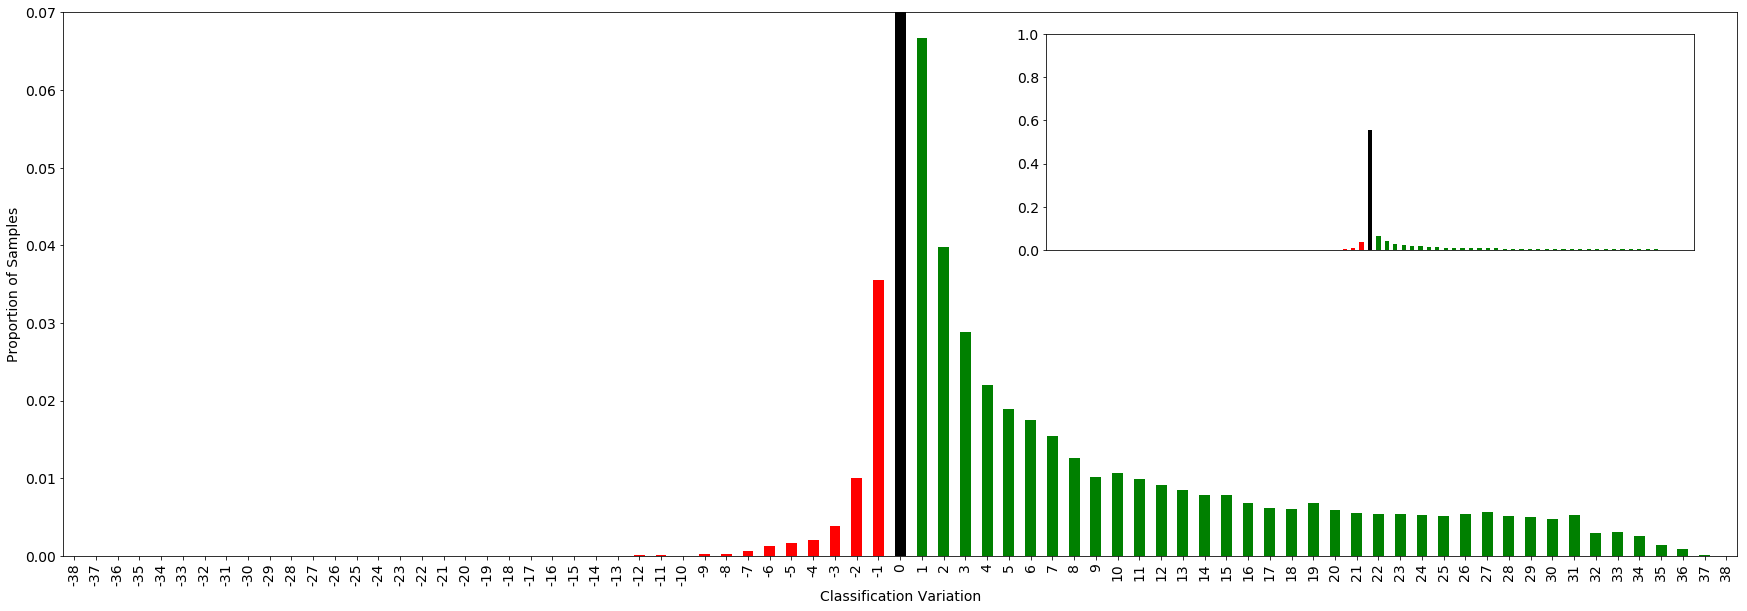
\includegraphics[width=\textwidth]{dups_frequency}
	\caption{Distribution of samples in terms of the changes in the number of positive classifications between last and first submissions, ($\Pl-\Pf$).}
	\label{fig:distribution_changes}
\end{figure*}

\medskip

Another interesting analysis on our dataset is understanding the vendors \emph{\gls{dr}} (or True Positive Rate), and \emph{\gls{fpr}}. 
Although these formulas are trivially defined respectively as
\begin{eqnarray}
\dr&=&\frac\tp{\#malware}=\frac\tp{\tp+\fn} \\ 
\fpr&=&\frac\fp{\#goodware}=\frac\fp{\tn+\fp}
\end{eqnarray}
%{\#goodware}, 
we lack ground truth for what is ${\#malware}$ and $\#goodware$.
To solve this, we propose relative metrics to compute what is positive ($\#malware$) and negative ($\#goodware$).


Our first approach is to take advantage of duplicated submissions to define an accuracy metric, $\Madups$.
As we have previously shown, 44.32\% of duplicated samples change in classification, which can be translated into vendors acknowledging their own errors.

With that in mind, for each vendor $v\in\VV$, we define a duplicated sample for $v$ (according to $\Madups$) as:
\begin{itemize}%[\IEEEsetlabelwidth{Z}]
	\item $\tp_v$, \emph{true positive for $v$}, if $v$ classified it positively in both the first and last submissions;
	\item $\tn_v$, \emph{true negative for $v$}, if $v$ classified it negatively in both the first and last submissions;
	\item $\fp_v$, \emph{false positive for $v$}, if $v$ classified it positively in the first submission and negatively in the last submission;
	\item $\fn_v$, \emph{false negative for $v$}, if $v$ classified it negatively in the first submission and positively in the last submission.
\end{itemize}

Figure~\ref{fig:dr_fpr_own} plots each vendors' $\dr_v$ vs.\ $\fpr_v$. We note that vendors do acknowledge their classification errors, as we see a detection rate from 56.82\% to 85.29\%, with a false positive rate ranging from 0.03\% to 6.91\%. 
Had they kept their original classification, one would have that $\Pl-\Pf = 0$ for every duplicate and consequently $\dr_v = 1$ and $\fpr_v = 0$. 
Notice that by keeping the original classification all clean samples remain clean, hence $\fn_v=0$, and all malicious samples remain malicious, hence $\fp=0$.

\begin{figure}[!h]
	\centering
	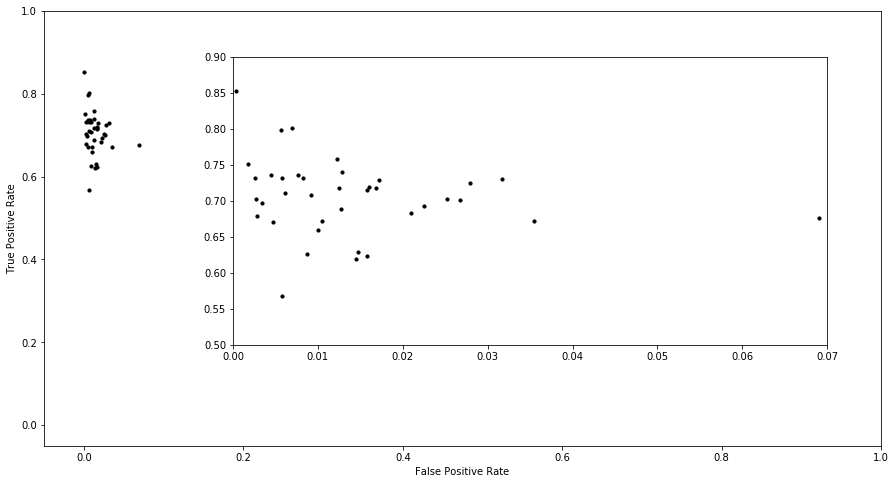
\includegraphics[width=\columnwidth]{dr_fpr_own}
	\caption{$\tpr_v$ vs. $\fpr_v$ according to $\Madups$.}
	\label{fig:dr_fpr_own}
\end{figure}

\medskip

For our second approach regarding vendors' accuracy, we take into account our observations from Figure~\ref{fig:distribution_changes} and our dataset $\CC$ to define another metric $\Mad$.

Intuitively a sample is classified as goodware according to this metric, \ie\ negative, if every vendor $v\in\mathcal{V}$ classifies it as clean.
To understand if our intuition is sound, we plot Figure~\ref{fig:distribution_clean}, a subset of Figure~\ref{fig:distribution_changes}, showing the frequency $\Pl-\Pf$ for samples that were classified as clean in their first submission, \ie, samples with $\Pf=0$. 
These account for 4,902 samples, 3,741 (76.32\%) of which do not increase in classification.

\begin{figure}[!h]
	\centering
	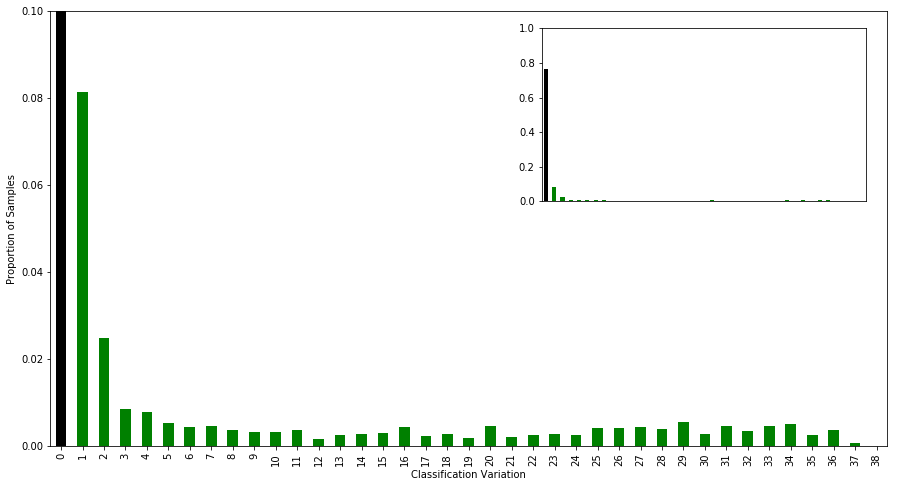
\includegraphics[width=\columnwidth]{distribution_clean}
	\caption{Distribution of samples that started as goodware and changed in the number of positive classifications between the last and first submission, \ie, $\Pl-\Pf$ for samples with $\Pf=0$}
	\label{fig:distribution_clean}
\end{figure}

To arrive at a positive (\ie\ malware) sample definition, we relate Figure \ref{fig:distribution_clean} with Figure \ref{fig:distribution_changes}.
Specifically we want to find a minimum threshold of positive classifications to define a sample as malware.
We chose five as the threshold, observing that percentage of samples that decrease in 5 or more positive classifications is 0.46\%, meaning it is an upper bound for samples that decrease from 5 or more to zero classifications. 

With the previous definitions, we can define a vendors' $v$ classification (according to $\Mad$) as:

\begin{itemize}%[\IEEEsetlabelwidth{Z}]
	\item $\tp_v$, \emph{true positive for $v$}, if $v$ and at least 5 other vendors in $\mathcal{V}$ classify it positively;
	\item $\tn_v$, \emph{true negative for $v$}, if $v$ and all other vendors in $\mathcal{V}$ classify it negatively;
	\item $\fp_v$, \emph{false positive for $v$}, if $v$ is the only vendor in $\mathcal{V}$ classifying it positively;
	\item $\fn_v$, \emph{false negative for $v$}, if $v$ classifies it negatively and at least 5 other vendors in $\mathcal{V}$ classify it positively.
\end{itemize}

Figure \ref{fig:dr_fpr_d} plots each vendors' $\dr_v$ vs. $\fpr_v$ according to~$\Mad$.
Using this metric we note that vendors' detection rate is more scattered than under $\Madups$, ranging from 20.17\% to 83.50\%, whereas false positive rate is similar, ranging from 0.01\% to 5.77\%.

\begin{figure}[!h]
	\centering
	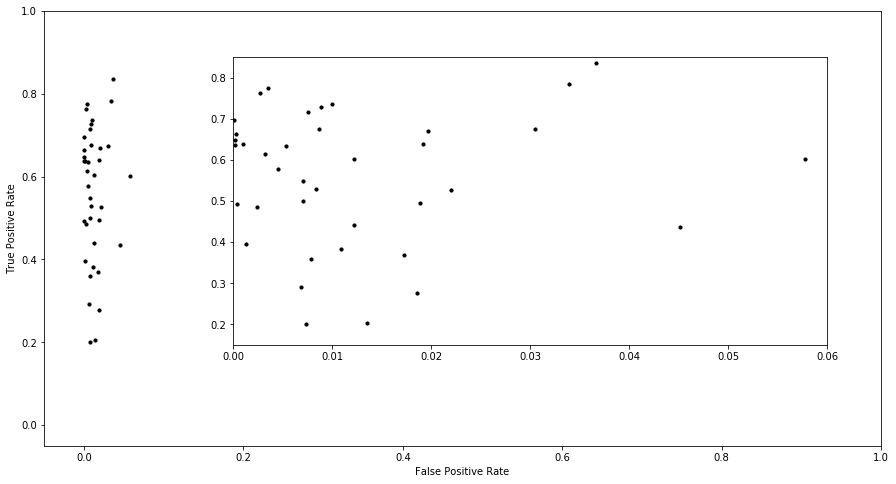
\includegraphics[width=\columnwidth]{dr_fpr_d}
	\caption{$\tpr_v$ vs. $\fpr_v$ according to $\Mad$.}
	\label{fig:dr_fpr_d}
\end{figure}

Given the impossibility of finding a source that is able to unanimously label each sample in our dataset, we want to find the vendors that perform the best under both metrics $\Madups$ and $\Mad$.
%We do so by filtering the top 20 vendors $\VVdups$ and $\VVd$, according to each metric and define $\VVstar=\VVdups\cap\VVd$.

Our approach to this problem is to filter the top 20 vendors $\VVdups$ and $\VVd$, according to each metric and define $\VVstar=\VVdups\cap\VVd$.
Given we have to maximize two variables, \tpr\ and \fpr, we decided to take advantage of the linear equation in the form $mx+b=y$ to choose the top vendors.
This form allows us to choose an $m$ and $b$ such that there are 20 vendors above the line, the top vendors $\VVstar$.
By tweaking the variable $m$ one can change the line's steepness, reflecting in a preference between \tpr\ and \fpr\:

\begin{itemize}
	\item \tpr\ preference: $m < 1$, less steepness therefore higher \fpr\ and \tpr\ values;
	\item \fpr\ preference: $m > 1$, more steepness, lower \fpr\ and \tpr\ values.
\end{itemize}

% Since we have no \emph{a priori} preference between $\tpr$ nor $\fpr$, we search for the maximum $b$ with $m=1$ such that there are exactly 20 vendors above $x+b=y$ in each graphic (Figures~\ref{fig:dr_fpr_own} and~\ref{fig:dr_fpr_d}).

Since we have no \emph{a priori} preference between $\tpr$ nor $\fpr$, we search for the maximum $b$ such that there are exactly 20 vendors above $x+b$ in each graphic (Figures~\ref{fig:dr_fpr_own} and~\ref{fig:dr_fpr_d}).

Figure \ref{fig:dr_fpr_top} shows the $\dr_v$ vs. $\fpr_v$ for the resulting 11 vendors under each metric, $\Madups$ in green and $\Mad$ in red, with $\dr_v$ varying from 63.49\% to 83.50\% and $\fpr_v$ from 0.01\% to 3.67\%.

\begin{figure}[!h]
	\centering
	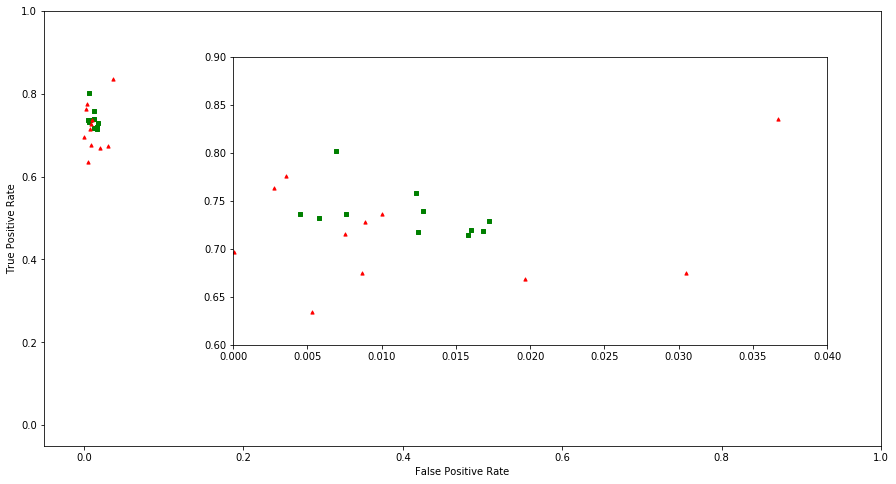
\includegraphics[width=\columnwidth]{dr_fpr_top}
	\caption{$\tpr_v$ vs. $\fpr_v$ according to $\Madups$ (green) and $\Mad$ (red).}
	\label{fig:dr_fpr_top}
\end{figure}


% To conclude the analysis of our datasets, we discuss the samples obtained from $\NSRL$~($\DNSRL$) and VirusShare.com~($\DVS$).
%We end this subsection with how the sets from \gls{nsrl} $\mathcal{D}_{NSRL}$ and VirusShare $\mathcal{D}_{VS}$ intersect our dataset $\mathcal{D}$. 
% Samples in $\DNSRL \cap \DD$ account for 4,756, while the number is 105,251 for $\DVS \cap \DD$. 

% Finally, and due to the ambiguity in the definition of malware, we also have that 426 samples are common to the three sets, \ie, are in $\DNSRL \cap \DVS \cap \DD$.

\subsection{Data Labelling}\label{sub_sec:data_labeling}
%%%%%%%%%%%%%%%%%%%%%%%%%%%%%%%%%%%%%%%%%%%%%%%
% From Data Labeling notebook
Having defined a collegiate set of vendors $\VVstar$ to classify the samples in our dataset, we can now turn our focus into labeling the reports as goodware or malware. 
To do so, we use $\CC$, together with $\NSRL$ and $\VS$, to derive three different metrics to label the reports as benign or malicious, over the set of vendors $\mathcal{V}^*$.

The first and most real metric we define is $\Mrealv$ that labels a sample $s\in\CC$ as:

\begin{itemize}
	\item $s\in\mal_\real$ if at least 5 vendors in $\VVstar$ classify $s$ positively;
	\item $s\in\good_\real$ if all vendors in $\VVstar$ classify $s$ negatively.
\end{itemize}

Since the labeling information is solely provided by $\VVstar$'s vendors, this metric's ground truth is highly dependent on their performance, which means labeling errors may be present (as we have discussed in \ref{sub_sec:data_analysis}). 
Due to this, samples that are classified positively by no more than four vendors, are discarded.

\medskip

Our second metric $\Mloosev$, restricts the previous metric $\Mrealv$ to achieve a better ground truth. We do this by including information from $\NSRL$ and VirusShare.com. 
This metric labels a sample $s\in\mathcal{C}$ as:

\begin{itemize}
	\item $s\in\mal_\loose$ if $s\in\mal_\real$ \textbf{and} it belongs to $\DVS$ and does not belong to $\DNSRL$;
	\item $s\in\good_\loose$ if $s\in\good_\real$ \textbf{and} it belongs to $\DNSRL$ and does not belong to $\DVS$.
\end{itemize}
that is
\begin{eqnarray*}
\mal_\loose&=&\left(\mal_\real\cap\DVS\right)\setminus\DNSRL\\
\good_\loose&=&\left(\good_\real\cap\DNSRL\right)\setminus\DVS
\end{eqnarray*}


By taking into account the presence in $\NSRL$, that reinforces cleanliness, and VirusShare.com, that reinforces maliciousness, this metric is more reliable, ground truth wise, at the expense of a smaller number of samples.

\medskip

Our third and final metric $\Mstrictv$, is the strictest one, labeling a sample $s\in\DD$ as:
\begin{itemize}
	\item $s\in\mal_\strict$ if all $v\in\VVstar$ classify it positively \textbf{and} $s\in\DVS\setminus\DNSRL$;
	\item $s\in\good_\strict$ if $s\in\good_\loose$.
\end{itemize}

Obviously this is the most reliable metric, in the sense that it is closely related to the samples' ground truth, leaving little room for disagreement. However, this is achieved again at the cost of a smaller number of samples.

\medskip

Taking the previously defined metrics, the task of creating labeled datasets based on them is trivial.
We apply each of the previously defined metrics, $\Mstrictv$, $\Mloosev$ and $\Mrealv$ to our classified dataset $\CC$ to obtained three new datasets, $\CC_{strict}\subseteq\CC_{loose}\subseteq\CC_{real}\subseteq\CC$.
Table \ref{tab:dataset_sizes} provides information regarding the size and number of malware and goodware in each of our datasets.

\begin{table}[!htb]
	\renewcommand{\arraystretch}{1.2} % more space between rows
	\centering
	\begin{tabular}{l|ccc}
		Dataset			& $\CC_{real}$ & $\CC_{loose}$ & $\CC_{strict}$	\\
		\hline
		Malware			& 98,582 & 45,306 & 24,658\\
		Goodware		& 56,475 & 1,989 & 1,989\\
		\hline
		Total			& 155,057 & 47,295 & 26,647\\
	\end{tabular}
	\smallskip
	\caption{Sizes for datasets $\CC_{real}$, $\CC_{loose}$ and $\CC_{strict}$.}
	\label{tab:dataset_sizes}
\end{table}

%!TEX root = main.tex
\color{black}
\section{Feature and Model Selection}\label{sec:feature_model}

In this subsection we describe our approach to feature selection and linear model choice.

\subsection{Feature Selection}
\label{section:feature_selection}

One of the most important stages in Machine Learning is the selection of the features to analyze, and features based on static imports have shown promising results in \gls{ml} applications for malware detection~\cite{miller:rev_int,schultz:data_mining}. 
In this section we describe the adopted static features that were fed into our model.

Although Cuckoo provides enormous amounts of usable information, we chose to start with simple features as to have a basic understanding of how doable our approach is.
More so, one of our main concerns is how the same feature gives different results under our different scenarios, hence the performance between scenarios and methodologies is more relevant than absolute performance.
With that in mind, we chose to use the static imports as features.

Using Celery~\cite{tool:celery}, a distributed task queue for Python, we optimized the parsing of the available HTML reports, extracting samples that contained information regarding static imports into a new set $\FF_{static}$.
We then joined the samples with static imports $\FF_{static}$ to the labeled samples $\CC_{real}$, obtaining a total of 155,057 labeled samples with static imports $\DD_{static} = \CC_{real} \cap \FF_{static}$.

We then vectorized imports by creating a binary vector where each position corresponds to a specific import.
If a given import $i$ is present in a sample, its feature vector $x$ will have the value 1 at that position $x_i$.
Likewise, if a given import $j$ is not present in a sample, its feature vector $x$ will have the value 0 at that position $x_j$.

Due to the amount of samples and variety of imports, each sample got a vector $x$ of 7,280 dimensions (\ie\ there are 7,280 different imports).
To reduce this number, and to remove any noise due to incorrect parsing of static imports by Cuckoo, we applied a variance threshold.

The variance threshold calculates the variance for each import, removing those that are below a given threshold.
In our case, since we are working with a binary vector, each import can be represented as Bernoulli random variable, hence their variance is given by $p(1-p)$.
With that in mind, we removed any import that did not vary in more than 99\% of samples.

The resulting dataset $\DD_{static}$ got reduced to 153,374 samples, each with a 64 dimensional binary vector.

\subsection{Model Selection}

In this subsection we go over the classifier used to create the model that separates malware from goodware.
Our main concerns when choosing a classifier regard the ability to produce a probabilistic output, good scaling for large number of features and samples, and ease of use.

Taking into consideration the guidelines given in~\cite{rossow:practices,shabtai:survey} and related work in~\cite{miller:rev_int,nissim:al_pdf,rieck:dynamic,schultz:data_mining}, we decide to use \textit{\acrfull{lr}} as our model.
This model fits our needs as it gives the probability of a random variable $X$ being 0 or 1, given a set of constraints (\ie~features), scales well with samples and features and it is readily available from several libraries, facilitating implementation~\cite{friedman2001elements}.

\gls{lr} can be defined with the form
\begin{eqnarray*}
	\rho(x) = \dfrac{1}{1 + e^{-x}},&x = \beta_0 + \beta_1x_1 + ... + \beta_nx_n
\end{eqnarray*}
where $\beta_n$ is the learned weight for feature $x_n$.
This weight is learned through iteration in order to minimize the error between the predicted values and the actual values.
In other words, given an \textit{n-th} dimensional set of features, \gls{lr} will try to create an hyperplane that divides samples from two classes.

As \gls{lr} is based on the logistic function (or sigmoid function), each feature $x_n$ can vary from $-\infty$ to $+\infty$ and still the output is contained between 0 and 1, hence providing probabilistic values.

%\todo[inline]{}
%\medskip 
%
%Our first and simplest model $\mathcal{LR}$, takes as features a sample's static imports, as a binary vector, and outputs the likelihood of a sample being malware. As we are dealing with a variety of malware samples, in the sense they have different behaviour and characteristics (\eg, trojan, virus), a generic classifier like this one may not perform well, as not only goodware may be diverse, but also is malware.
%
%\medskip
%
%To mitigate this shortcoming we provide a more complex model $\mathcal{E}$, which comprises a simple ensemble stacking approach. This model also takes as features the static imports and outputs the likelihood of a sample being malware, but it is layered in two steps.
%
%The first step (layer $\mathcal{E}_{\mathcal{L}_{0}}$) is composed of 6 \gls{lr} models, where each model is trained to output the likelihood of a sample belonging to one of six classes: trojan $\mathcal{C}_{t}$, worm $\mathcal{C}_{w}$, virus $\mathcal{C}_{v}$, spyware $\mathcal{C}_{s}$, ransom $\mathcal{C}_{r}$, or other $\mathcal{C}_{o}$, in a \textit{one-vs-all} methodology, \ie, a sample either belongs to $\mathcal{C}_{n}$ or not, with a sample's static imports as features.
%
%%\todo[inline]{maybe talk about AVClass here. PA: concordo}
%%\todo[inline]{\color{blue}moved to III-B.}
%
%The second step (layer $\mathcal{E}_{\mathcal{L}_{1}}$) is identical to $\mathcal{LR}$, but now takes as features the output of each classifier from the previous layer, outputting the likelihood of a sample being malware.
%
%In summary, we make use of two models $\mathcal{LR}$ and $\mathcal{E}$, both using a linear logistic regression as base, but where $\mathcal{LR}$ uses a single classifier, and $\mathcal{E}$ uses a 2 layer ensemble stacking with 6 classifiers on the first layer providing input to a single classifier in the second layer, with the hope of facilitating class separation.
%!TEX root = main.tex
\color{black}
\section{Evaluation and Results}\label{sec:eval_results}

In this section we aim at doing a comparative analysis on three different scenarios $\mathcal{S}_{\strict}$, $\mathcal{S}_{\loose}$ and $\mathcal{S}_{\real}$, built on top of the previously defined metrics. This comparison is done using standard cross-validation methodologies and a proposed temporal-based methodology.

We further provide an analysis on how to reduce the size of the training set, without compromising the final results.

\subsection{Evaluation}

With regards to our evaluation methodology, as we have previously mentioned, our purpose is to understand how laboratory conditions compare to real-world conditions.
We now detail how we achieve and compare these conditions.

Given the purpose of our work, we choose to measure our results by plotting an \gls{auroc} graph, which measures the \tpr~at different \fpr~levels, metrics that are commonly used across similar work~\cite{miller:rev_int,nissim:al_pdf,schultz:data_mining}.

The three scenarios that we will focus on will rely on metrics $\Mrealv$, $\Mloosev$ and $\Mstrictv$, over the dataset $\DD$:

\begin{itemize}
	\item Real Scenario $\mathcal{S}_{\real}$, applies the metric $\Mrealv$, containing 98,582 malware samples and 56,475 goodware samples.
	\item Loose Scenario $\mathcal{S}_{\loose}$, applies the metric $\Mloosev$, containing 45,306 malware samples and 1,989 goodware samples.
	\item Strict Scenario $\mathcal{S}_{\strict}$, applies the metric $\Mstrictv$, containing 24,658 malware samples and 1,989 goodware samples.
\end{itemize}

Given these three scenarios, we consider the following evaluation metrics:

\paragraph{Cross-validation (Figure \ref{fig:dia_xvalidation})}
To gain insight on how each model generalizes our scenarios, we apply a k-fold cross-validation, with $k=10$. This methodology splits the dataset into $k$ subsets (\ie, folds), selecting a single fold for validation and the remaining $k-1$ folds for training. This process is repeated $k$ times, ensuring every fold is used for validation and training.

\begin{figure}[!h]
	\centering
	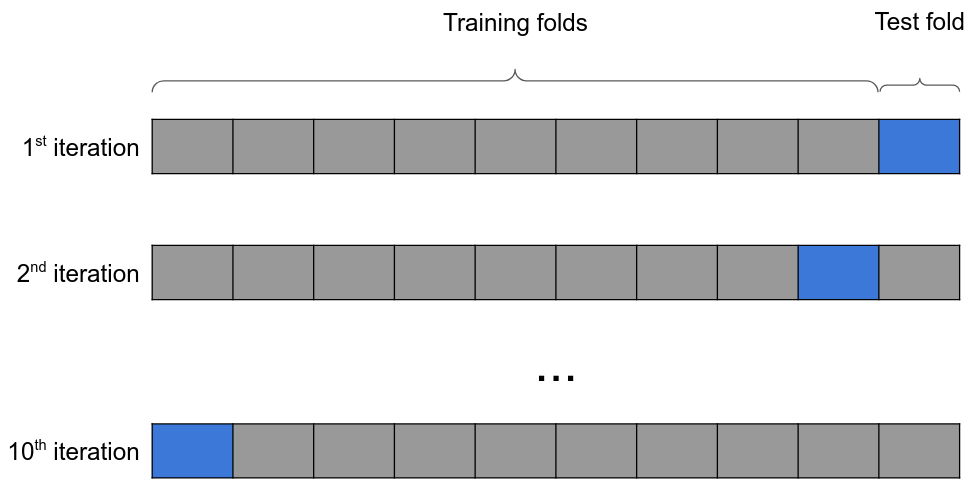
\includegraphics[width=\columnwidth]{dia_xvalidation}
	\caption{Cross-Validation evaluation example with 10 folds.}
	\label{fig:dia_xvalidation}
\end{figure}

Although the cross-validation methodology enables to measure the generalization capabilities of a model, it does not account for temporal ordering of the samples. Since we want to measure the score when training samples pre-date the validation samples, we now define a couple of temporal based validations. These are validated on the best performing model from cross-validation for all 3 scenarios.

\paragraph{Temporal based validation}
The first temporal based validation, which we designate as \textit{Past-to-Present validation}, Figure~\ref{fig:dia_pastpresent}, can be resumed as an iterative methodology where the validation set is fixed with the most recent samples, and the training set with the oldest. At each iteration the training set is extended with more recent samples and scored against the validation, until all samples are used.

\begin{figure}[!h]
	\centering
	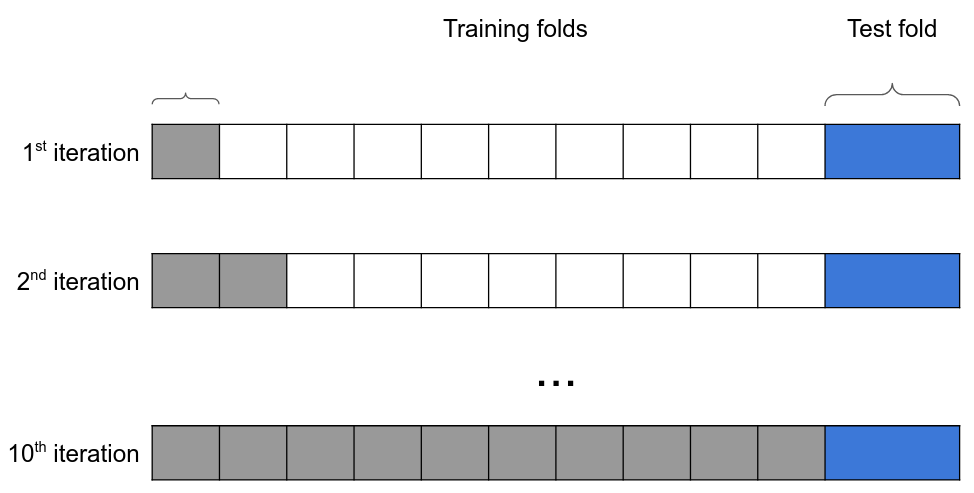
\includegraphics[width=\columnwidth]{dia_pastpresent}
	\caption{Past-to-Present evaluation example with 20/80 test/training, 10 folds in training.}
	\label{fig:dia_pastpresent}
\end{figure}


The second temporal based validation, which we designate as \textit{Present-to-Past validation}, Figure~\ref{fig:dia_presentpast}, is the opposite of \textit{Past-to-Present} with regards to the starting position of the training set. Again the validation is fixed the most recent samples, but now the training set starts with the temporally closest samples to the validation set. At each iteration the training set is extended, this time with older samples and scored against the validation, until all samples are used.

\begin{figure}[!h]
	\centering
	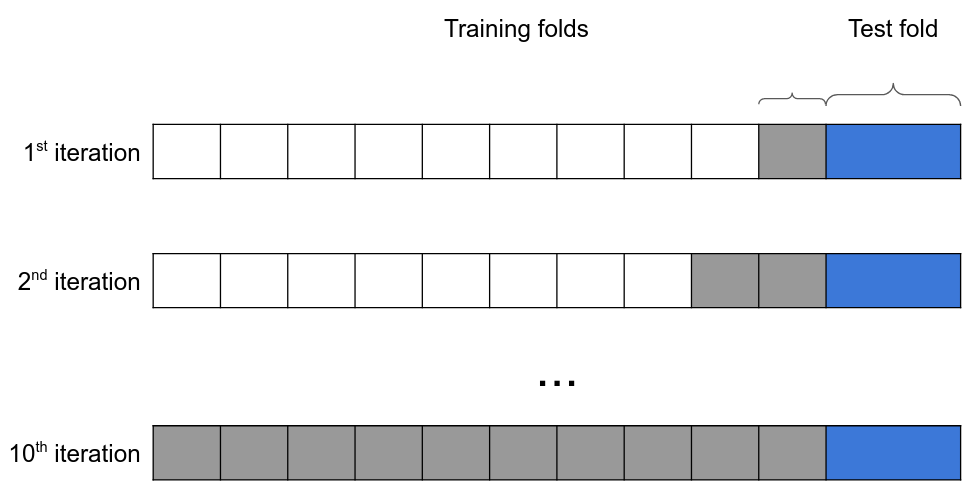
\includegraphics[width=\columnwidth]{dia_presentpast}
	\caption{Present-to-Past evaluation example with 20/80 test/training, 10 folds in training.}
	\label{fig:dia_presentpast}
\end{figure}

\textit{Past-to-Present} and \textit{Present-to-Past} validations both require two parameters, specifically the size of the validation set, and how the increments to the training set are made. For our evaluation, we use the 20\% most recent samples as validation, and split the remaining 80\% into 10 folds, hence the validation is done 10 times, with each iteration increasing the training size by one fold.

These two validation methodologies give us the ability to account for temporal consistency. Moreover, they enable us to compare the importance of older \textit{vs} newer samples to classify recent samples.

We designate the third and last temporal based validation as \textit{Temporal Window validation}, Figure~\ref{fig:dia_slidingwindow}. This validation methodology is inspired on regular cross-validation, in the sense that it splits the dataset into folds, but changes how the folds are used. Specifically it takes $n$  temporal consistent and contiguous folds, \ie, each fold immediately precedes the next one, and uses the last fold (more recent samples) for validation, and the previous folds for training (older samples). By starting with the $n$ first folds and sliding one fold on each iteration, we apply a sliding window of size $n$ over the dataset.

\begin{figure}[!h]
	\centering
	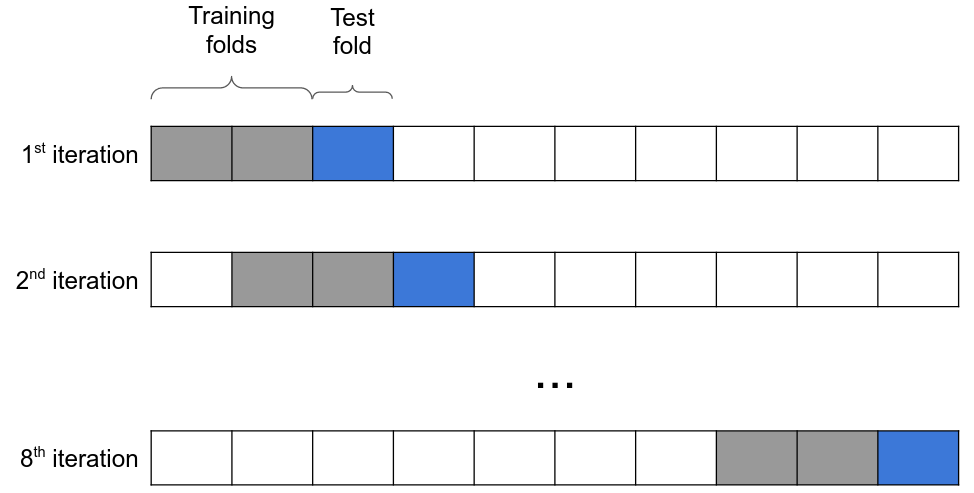
\includegraphics[width=\columnwidth]{dia_slidingwindow}
	\caption{Temporal window evaluation example with window of size 3 over a 10 fold dataset.}
	\label{fig:dia_slidingwindow}
\end{figure}

For this last validation methodology, we again split the dataset into 10 folds. The sliding window size, $n$, is chosen during the results phase, as its choice depends on previous results.

We measure the \gls{auroc} during each validation's iteration and use the average measurement to discuss the results.

\subsection{Results}
\label{section:single_layer_results}

We implement our experiments in Python, by using Jupyter Interactive Notebooks\cite{tool:jupyter} to facilitate data visualization. We use scikit-learn\cite{tool:sklearn} for \gls{ml}, and Pandas\cite{tool:pandas} for data analysis. Our experiments were conducted on an Ubuntu Virtual Machine with 16 cores and 16GB of RAM, in order to minimize training and validation times.

We now focus on applying the evaluation methodologies to our scenarios. This enables us to compare the different conditions, and consequently results, that affect malware detection.

%We compare each model $\mathcal{LR}$ and $\mathcal{E}$ under each scenario $\mathcal{S}_{\strict}$, $\mathcal{S}_{\loose}$ and $\mathcal{S}_{\real}$.

We start with what we determine as \textit{laboratory conditions}, ideal conditions for the problem of malware detection. These are met when we apply the strict metrics $\Mstrictv$, to the dataset $\mathcal{C}$, obtaining scenario $\mathcal{S}_{\strict}$.

Under these conditions, our model provides the best results, with an \gls{auroc} of 0.91, as shown by the red curve in Figure \ref{fig:xval_results}. We argue that such high values are easily attained from factors like a small and reliable dataset, and the use of cross-validation, which mixes samples and ignores possible dependencies on malware samples.

\begin{figure}[!h]
	\centering
	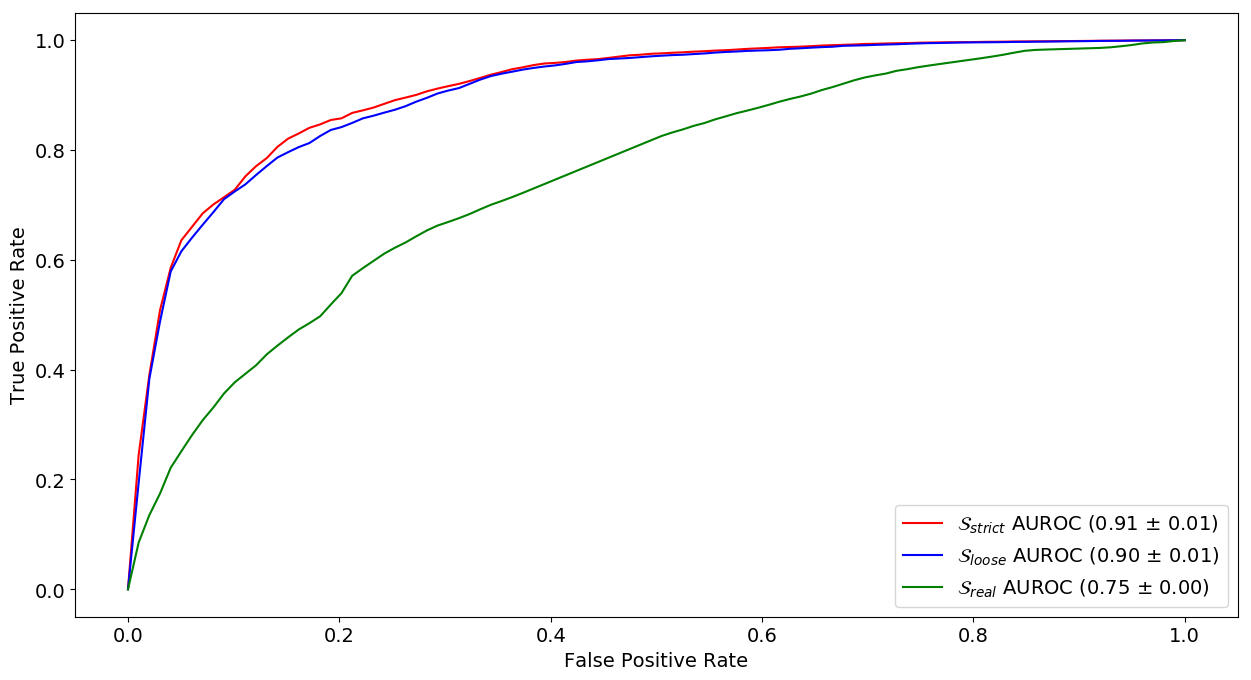
\includegraphics[width=\columnwidth]{xval_results}
	\caption{Cross-Validation \gls{roc} and \gls{auroc} for our model under $\mathcal{S}_{\strict}$, $\mathcal{S}_{\loose}$ and $\mathcal{S}_{\real}$.}
	\label{fig:xval_results}
\end{figure}

To understand how reliability influences the models' result, we use scenarios $\mathcal{S}_{\loose}$ and $\mathcal{S}_{\real}$, which are less reliable and include more samples.

Under these more relaxed, \textit{real-world} conditions, the model's results hold an \gls{auroc} of 0.90 under $\mathcal{S}_{\loose}$, as shown by the blue curve in Figure \ref{fig:xval_results}, and an \gls{auroc} of 0.75 under $\mathcal{S}_{\real}$, as seen by the green curve in Figure \ref{fig:xval_results}.

From $\mathcal{S}_{\strict}$ to $\mathcal{S}_{\loose}$, the only change is the amount of malware labeled samples, which significantly increase.
The difference is interesting, as although the number of malware labeled samples increase significantly, the results are not that affected.
This suggests that although the reliability for malware decreases, its impact is not as noticeable as expected.
This might also suggest that vendors do converge on their definition of malware, under our $\Mloosev$ metric.
If vendors did not converge on what is malware, adding more samples would culminate in worse results, as separation between malware and goodware would become harder.

When looking at the changes from $\mathcal{S}_{\loose}$ to $\mathcal{S}_{\real}$, not only the amount of malware labeled samples increase, but also the number of goodware labeled samples, both by a significant amount. 
The way this impacts the results is pretty significant, as we observe a high decrease in the \gls{auroc}.
The metric $\Mrealv$ that labels malware and goodware for this scenario $\mathcal{S}_{\real}$ disregards the cross-check from outside repositories, which in turn degrade the reliability significantly, as well as increase the dataset size notably.
We attribute the results' degradation mainly to the unreliability of goodware labeling, not only because we have previously seen that increase in malware does not significantly impact results (from $\mathcal{S}_{\strict}$ to $\mathcal{S}_{\loose}$), but also due to the tendency for false negatives in vendors (Figure \ref{fig:distribution_changes}), which in turn lead us to incorrectly label goodware for the samples in $\mathcal{C}$.

The results we described show how moving from \textit{laboratory conditions} to more \textit{real-world conditions} degrade the model's performance. We now focus on using our previously defined temporal based methodologies to further converge into a real-world scenario.

\medskip

We start by applying our \textit{Past-to-Present} validation to the three scenarios, $\mathcal{S}_{\strict}$, $\mathcal{S}_{\loose}$ and $\mathcal{S}_{\real}$.
As previously defined, this validation starts with an older set of training samples and iteratively adds newer samples, validating each iteration on a fixed set of the most recent samples.
Since our interest is to measure performance variation over time, we plot in Figure~\ref{fig:pastpresent} the \gls{auroc} at every iteration (\ie, fold), for each of our three scenarios.

\begin{figure}[!h]
	\centering
	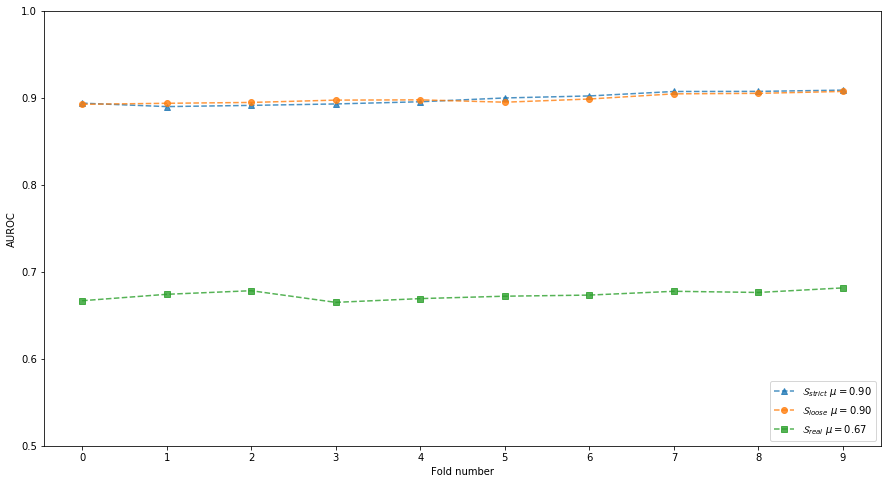
\includegraphics[width=\columnwidth]{pastpresent}
	\caption{\gls{auroc} for each iteration of the \textit{Past-to-Present} evaluation. Folds order consistent with temporal order (\ie, fold 0 contains older samples than fold 1)}
	\label{fig:pastpresent}
\end{figure}

When directly comparing the average \gls{auroc} for cross-validation and our \textit{Past-to-Present} validation, we note that for both $\mathcal{S}_{\strict}$ and $\mathcal{S}_{\loose}$ the \gls{auroc} remains identical, while for $\mathcal{S}_{\real}$ the score decreases from 0.75 to 0.67.
This decrease is intuitive to the methodology, as we are forcing temporal consistency between samples.

For both $\mathcal{S}_{\strict}$ and $\mathcal{S}_{\loose}$ we note only a slight increase as new folds are added.
They still relate, as we have previously noted for cross-validation, arguably given their metrics $\Mstrictv$ and $\Mloosev$ are not very different.
The small variation to the cross-validation methodology can be justified by using small dataset size for both cases.

As for $\mathcal{S}_{\real}$ we note higher variation and lower overall score, as the reliability of the metric $\Mrealv$ goes down.
This is expected, not only because we are enforcing temporal consistency between samples, but as new folds are added, the training gets bigger, while the test remains the same.

Our main observation for this validation methodology is that there is a slight tendency for \gls{auroc} to increase, as we move forward in time, close to the validation set.

From these observations, we argue about the possibility that with fixed validation set of the most recent samples, a model benefits by using samples temporally closer to validation.

\medskip

Our next result, which uses our \textit{Present-to-Past} validation methodology will further help analyze the aforementioned detail.
The \textit{Present-to-Past} validation enhances the previous results under real-world conditions. 
This methodology starts by fixing the validation set to the most recent samples, but with the training set starting at the temporally closest samples to validation.
At each iteration, older samples are added to the training set and validated on the fixed, most recent, samples.

By applying this methodology to the three scenarios, $\mathcal{S}_{\strict}$, $\mathcal{S}_{\loose}$ and $\mathcal{S}_{\real}$, we plot Figure \ref{fig:presentpast}, where the X axis increases as older samples are added to the training set (\eg\ fold 0 contains newer samples than fold 1), hence measuring the performance variance over time. Similarly to the previous observation, the average \gls{auroc} suffers a decrease when compared to cross-validation.
For $\mathcal{S}_{\strict}$ we note a change from 0.91 to 0.90, for $\mathcal{S}_{\loose}$ the score is the same, and for $\mathcal{S}_{\real}$ 0.75 to 0.69.

\begin{figure}[!h]
	\centering
	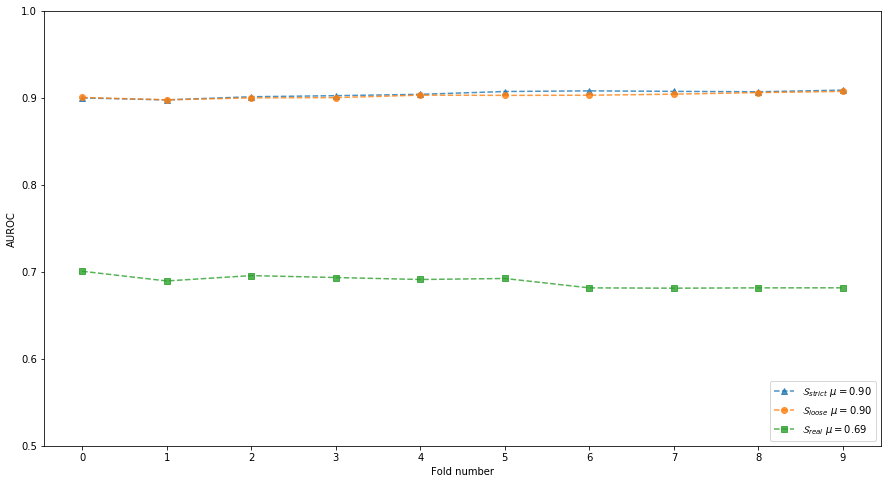
\includegraphics[width=\columnwidth]{presentpast}
	\caption{\gls{auroc} for each iteration of the \textit{Present-to-Past} evaluation. Folds order is the inverse of temporal order (\ie, fold 0 contains newer samples than fold 1)}
	\label{fig:presentpast}
\end{figure}

The comparison between scenarios is identical to what was observed in cross-validation and \textit{Past-to-Present}: scenarios $\mathcal{S}_{\strict}$ and $\mathcal{S}_{\loose}$ display very similar results, with $\mathcal{S}_{\real}$ dropping behind due to its less reliable labeling metric.
It is noticeable that using the entire dataset does not bring much improvement to the final results. In fact, for $\mathcal{S}_{\real}$ the score even drops after fold $\#2$.

With these results, our original observation that samples closer to the validation set benefit the model becomes more convincing. In fact, we argue that there should be an ideal number of necessary training folds, temporally consistent with the validation fold (\ie\ any fold from training predates validation), needed to maximize the overall score.

\medskip

Finally, we analyze how does such reduced training set behaves in our scenarios; for this purpose, we define a sliding window that moves forward in time through each scenario for training and validation.
We propose a reduction on the training size to $n=3$ folds predating the validation fold.
We choose $n = 3$, since we have seen that the scores either do not improve (for $\mathcal{S}_{\strict}$ and $\mathcal{S}_{\loose}$) or actually go down (for $\mathcal{S}_{\real}$) with higher folds.
In summary, we have selected 30\% of each dataset for training purposes and the next 10\% for validation (3 training folds, 1 validation fold), and then started moving the window forward in time (1 fold at a time) to obtain the following results (Figure~\ref{fig:slidingwindow}): for  $\mathcal{S}_{\strict}$, $\mathcal{S}_{\loose}$ and $\mathcal{S}_{\real}$, we obtain \gls{auroc} values of 0.89, 0.88 and 0.76, respectively. 
These results come to reaffirm our argument that we can reduce the size of the training set, without losing any significant score.

\begin{figure}[!h]
	\centering
	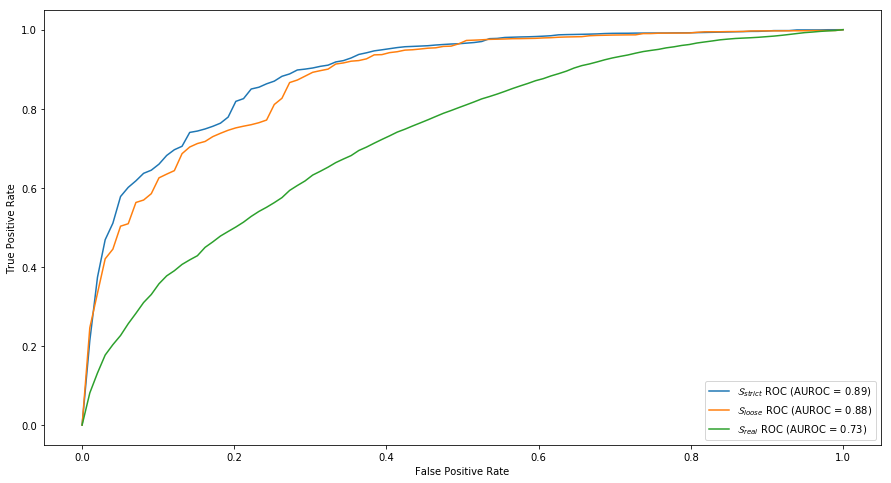
\includegraphics[width=\columnwidth]{slidingwindow}
	\caption{\gls{roc} and \gls{auroc} for our three scenarios, under the \textit{Temporal Window} methodology.}
	\label{fig:slidingwindow}
\end{figure}

Comparing these results with the baseline cross-validation, we note a decrease for each scenario, specifically a decrease from 0.91 to 0.89 for $\mathcal{S}_{\strict}$, from 0.90 to 0.88 for $\mathcal{S}_{\loose}$ and from 0.75 to 0.73 for $\mathcal{S}_{\real}$.
We should highlight that the results that use temporal consistency should better reflect the reality than standard cross-validation, since we are requiring temporally ordered samples.
Another important idea that should be stressed is that for cross validation we used a fairly reasonable amount of data for training purposes, whereas in this last case we used a restricted amount of data. This might be a relevant issue in a few year's time. The results obtained are summarized in Table \ref{tab:singlelayer_results}.

\begin{table}[!htb]
	\renewcommand{\arraystretch}{1.2} % more space between rows
	\centering
	\begin{tabular}{l|cccc}
		AUROC & $\DS_\strict$ & $\DS_\loose$ & $\DS_\real$ & Train/Test \%\\
		\hline
		Cross-Validation & 0.91 & 0.90 & 0.75 & 90 / 10\\
		Past-to-Present & 0.90 & 0.90 & 0.67 & 10 to 90 / 10\\
		Present-to-Past & 0.90 & 0.90 & 0.69 & 10 to 90 / 10\\
		Sliding-Window & 0.89 & 0.88 & 0.73 & 30 / 10\\
		\hline
	\end{tabular}
	\smallskip
	\caption{Single layer results summary.}
	\label{tab:singlelayer_results}
\end{table}

\medskip

With a better understanding of how the model behaves under different methodologies, we now diverge to how we improved not only the overall results, but also the information provided by the model.

%!TEX root = main.tex

\section{Model Improvements}
\label{sec:improvements}

Having a solid baseline model for our malware detection task together with how laboratory \textit{vs.}\ real-world scenarios change the model outcome, we now take this section to present the improvements made in order to obtain a more robust model to detect malware.
We start by describing our first improvement, applying a multi layer model to extract more information regarding a sample.
We then take this enhanced model and increase the number of features to include dynamic content and how it impacted the model's results.

%%%%%%%%%%%%%%%%%%%%%%%%%%%%%%%%%%%%%%%%%%%%%%%%%%%%%%%%%%%%%%%%%%%%%%%%
\subsection{Multi Layer Model}
\label{section:improvements_multi_layer}

On the previous chapter we ended up with a simple \gls{lr} model $\LR$ that given a set of static imports from a sample, would give the probability of it being malware.

In this section we provide a new model $\mathcal{E}$ comprises a simple ensemble stacking approach, which instead of using a single \gls{lr} classifier, multiple ones are used, layered into two steps.

The first step (layer $\mathcal{E}_{\mathcal{L}_{0}}$) is composed of $n$ \gls{lr} models, where $n$ is the number of possible classes.
Each model is trained to output the likelihood of sample belonging to one of the $n$ classes, in a \textit{one-vs-all} methodology (\ie\ a sample either belongs to $\mathcal{C}_{n}$ or not), having as input the raw features (\eg\ static imports).

The second step (layer $\mathcal{E}_{\mathcal{L}_{1}}$) is identical to $\mathcal{LR}$, but now takes as features the output of each classifier from the previous layer, outputting the likelihood of a sample being malware.

In summary, as depicted in Figure \ref{fig:dia_multilayer}, we define a 2 layer ensemble stacking with $n$ classifiers on the first layer to a single classifier in the second layer.

\begin{figure}[h]
	\centering
	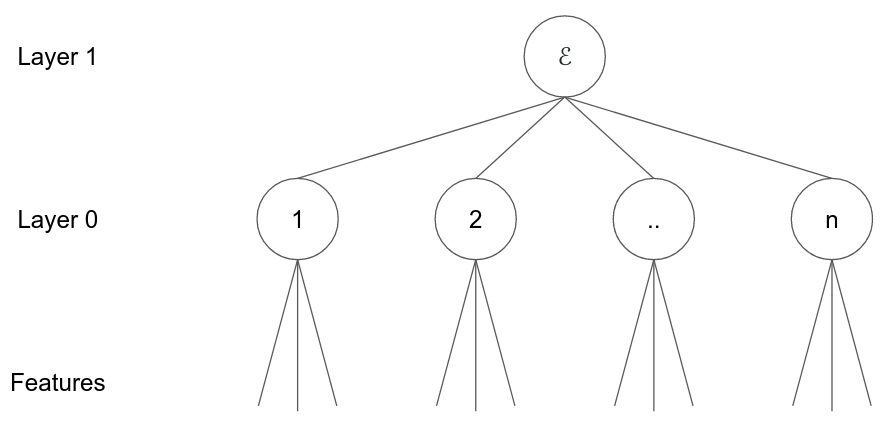
\includegraphics[width=\columnwidth]{dia_multilayer}
	\caption{Multi layer model representation.}
	\label{fig:dia_multilayer}
\end{figure}

%%%%%%%%%%%%%%%%%%%%%%%%%%%%%%%%%%%%%%%%%%%%%%%%%%%%%%%%%%%%%%%%%%%%%%%%
\subsection{Malware Classes}

We now present our approach on selecting the $n$ classes of interest.
This represents another labeling problem, but now instead of having to label between goodware and malware, we have to label the malware as belonging to some subclass.

With this in mind, we chose 6 malware classes: \textit{virus}, \textit{trojan}, \textit{worm}, \textit{ransom}, \textit{spyware} and \textit{other}.

To help label our malware samples into the aforementioned classes, we take a tool by Sebastián, M. et al.~\cite{sebastian2016avclass}, AVClass, which was built to normalize a malware sample name into the most likely family, and modify it such that instead of providing a family name, it would provide one (or more) of the 6 previously defined classes.
Specifically, we changed it in a way that given a set of malware names, the output would be a distribution over the 6 malware classes.

To calculate each class weight we apply the following formula
\begin{eqnarray*}
	\mathcal{W}_c = \dfrac{f_c}{\sum\limits_{c}f_c}
\end{eqnarray*}

where $f_c$ is the frequency for the class $c$ and $\sum_{c}f_c$ is the number of times all classes appear.
For example, if a given set of names contain the name \textit{trojan} 3 times and the name \textit{virus} one time, then the weights would be

\begin{eqnarray*}
	\mathcal{W}_{trojan}=\dfrac{3}{4}=0.75,~\mathcal{W}_{virus}=\dfrac{1}{4}=0.25,\\\mathcal{W}_{c}=0, c \in \{worm, spyware, other, ransom\}
\end{eqnarray*}

\medskip

Having these malware classes defined for our multi layer model, we also added the \textit{goodware} class for samples that are not malware.
Doing so gives us 7 possible classes, 6 of which are malware only.
It is worth mentioning that if a sample belongs to the \textit{goodware} class, it cannot belong to any other, likewise, if it belongs to any malware class, it cannot belong to the \textit{goodware} class.
Table \ref{tab:dataset_sizes_new} discriminates the amount of each malware class.

\begin{table}[!htb]
	\renewcommand{\arraystretch}{1.2} % more space between rows
	\centering
	\begin{tabular}{lccc}
		Dataset			& $\CC_{real}$ & $\CC_{loose}$ & $\CC_{strict}$	\\
		\hline
		Trojan			& 97,054 & 44,329 & 24,176\\
		Other			& 49,443 & 24,126 & 14,750\\
		Worm			& 24,554 & 14,837 & 9,381\\
		Virus			& 21,055 & 12,531 & 6,899\\
		Spyware			& 20,724 & 10,172 & 5,955\\
		Ransom			& 7,761 & 1,924 & 1,160\\
		\hline
		\hline
		Malware Total	& 98,582 & 45,306 & 24,658\\
		\hline
	\end{tabular}
	\medskip
	\caption{Samples belonging to each of the 6 malware classes for $\CC_{real}$, $\CC_{loose}$ and $\CC_{strict}$.}
	\label{tab:dataset_sizes_new}
\end{table}

\medskip

In the base model, we used static imports as features for our malware detection model.
Although the results are reasonable, the information which can be retrieved from static imports alone is limited.
As an example, if a sample is compressed, encrypted or packed, its behavior cannot be inferred from static imports only.
To overcome these limitations, we resort to more dynamic information provided by Cuckoo.

%%%%%%%%%%%%%%%%%%%%%%%%%%%%%%%%%%%%%%%%%%%%%%%%%%%%%%%%%%%%%%%%%%%%%%%%
\subsection{Category Calls}
\label{section:improvements_categories}

The first type of dynamic information we extracted were the number of dynamic category calls.
When Cuckoo runs and monitors a sample, it registers some low level library calls, which it then assigns to a fixed number of categories.

There are a total of 14 different categories defined by Cuckoo: \textit{anomaly}, \textit{device}, \textit{filesystem}, \textit{hooking}, \textit{misc}, \textit{network}, \textit{process}, \textit{registry}, \textit{services}, \textit{socket}, \textit{synchronization}, \textit{system}, \textit{threading} and \textit{windows}.
After using Celery~\cite{tool:celery} to extract the number of each category calls for the samples, we obtained a total of 148,036 samples with information regarding category calls.

To normalize the category calls value, we decide to transform the values to follow a normal distribution.
We do this by using scikit-learn's~\cite{tool:sklearn} \textit{QuantileTransformer} with a normal distribution, which splits the possible values into bins such that the resulting distribution is of type \textit{Gaussian} with a mean of 0.
This way we have a greater number of bins around the mean, allowing for better discrimination, whereas very large values fall into the same bin.

%%%%%%%%%%%%%%%%%%%%%%%%%%%%%%%%%%%%%%%%%%%%%%%%%%%%%%%%%%%%%%%%%%%%%%%%
\subsection{Library Calls}
\label{section:improvements_api_unigrams}

Our second type of dynamic information are the number of library calls.
While \textit{category calls} provide the number of calls for a given category, \textit{library calls} provide the count for each library call, hence being a subset of the previous.

Cuckoo~\cite{tool:cuckoo} registers the number of calls for 163 different functions, ranging from opening and closing files, to opening and closing sockets.
Again we used Celery~\cite{tool:celery} to extract these numbers, obtaining information from 148,036 samples.

Given we are dealing with a high number of features (163 different library calls), we decided to apply the same variance threshold as in Section \ref{section:feature_selection}, to remove features that do not vary in most samples.
By choosing a threshold of 80\%, we remove library calls that do not vary in more than 80\% of the samples, effectively reducing the number of library calls to 144.
With regards to how these features can vary from 0 to $+\infty$, as before, we again apply a quantile transformer with a normal distribution.

%%%%%%%%%%%%%%%%%%%%%%%%%%%%%%%%%%%%%%%%%%%%%%%%%%%%%%%%%%%%%%%%%%%%%%%%
\subsection{Cuckoo Signatures}
\label{section:improvements_signatures}

For our third and last type of dynamic information, we resort to Cuckoo's~\cite{tool:cuckoo} custom signatures.
These signatures are built from certain activities that Cuckoo deems malicious or suspicious.
For example, if a sample allocates memory and then makes it executable, it might suggest some sort of packing or obfuscation.

To extract these signatures, we use Celery~\cite{tool:celery} and obtain a total of 124,821 samples and 61 different signatures.
As with our static import features, we use a binary vector for each sample, where each position corresponds to a specific signature. Re-iterating on how we represent this, if a given signature $i$ is present in a sample, its feature vector $x$ will have the value 1 at that position $x_i$. Likewise, if a given signature $j$ is not present in a sample, its feature vector $x$ will have the value 0 at that position $x_j$.

\medskip

We joined these features $\FF_{dynamic}$ to the labeled samples $\CC_{real}$, obtaining a total of 122,633 labeled samples with the new features $\DD_{dynamic} = \CC_{real} \cap \FF_{dynamic}$.

Given there is a lower amount of available samples, we provide in Table \ref{tab:dataset_sizes_improved} the new sizes for $\CC_{real}$, $\CC_{loose}$ and $\CC_{strict}$, which take into account the new features $\FF_{dynamic}$.

\begin{table}[!htb]
	\renewcommand{\arraystretch}{1.2} % more space between rows
	\centering
	\begin{tabular}{lccc}
		Dataset			& $\CC_{real}$ & $\CC_{loose}$ & $\CC_{strict}$	\\
		\hline
		Malware			& 94,248 & 42,911 & 23,437\\
		Goodware		& 28,385 & 1,741 & 1,741\\
		\hline
		Total			& 122,633 & 44,652 & 25,178\\
		\hline
	\end{tabular}
	\medskip
	\caption{New sizes for datasets $\CC_{real}$, $\CC_{loose}$ and $\CC_{strict}$.}
	\label{tab:dataset_sizes_improved}
\end{table}

%%%%%%%%%%%%%%%%%%%%%%%%%%%%%%%%%%%%%%%%%%%%%%%%%%%%%%%%%%%%%%%%%%%%%%%%
\section{Improved Model Results}
\label{section:improvements_results}

We now present the results of our new model $\mathcal{E}$, validated using the same methodology as described in \ref{sec:eval_results}.

Specifically we test the model using the baseline cross-validation methodology, followed by our three temporally consistent scenarios: \textit{Past-to-Present}, \textit{Present-to-Past} and \textit{Temporal Window}.
We test each methodology using the three different scenarios: $\mathcal{S}_{\strict}$, $\mathcal{S}_{\loose}$ and $\mathcal{S}_{\real}$.
\medskip

Starting with \textit{laboratory conditions}, we apply the cross-validation evaluation to model $\mathcal{E}$ with the labeled dataset $\CC_{strict}$ and features $\DD_{dynamic}$, providing scenario $\mathcal{S}_{\strict}$.
For this scenario, we obtain an \gls{auroc} of 98\%, as presented by the red curve in Figure \ref{fig:improved_xval}.

Relaxing to more \textit{real-world conditions}, under the form of a less reliable ground truth, we test the datasets $\CC_{loose}$ and $\CC_{real}$ on features $\DD_{dynamic}$.
As shown in Figure \ref{fig:improved_xval}, the score under \gls{auroc} is 98\% for $\mathcal{S}_{\loose}$ (blue curve) and 95\% for $\mathcal{S}_{\real}$ (green curve).

\begin{figure}[!h]
	\centering
	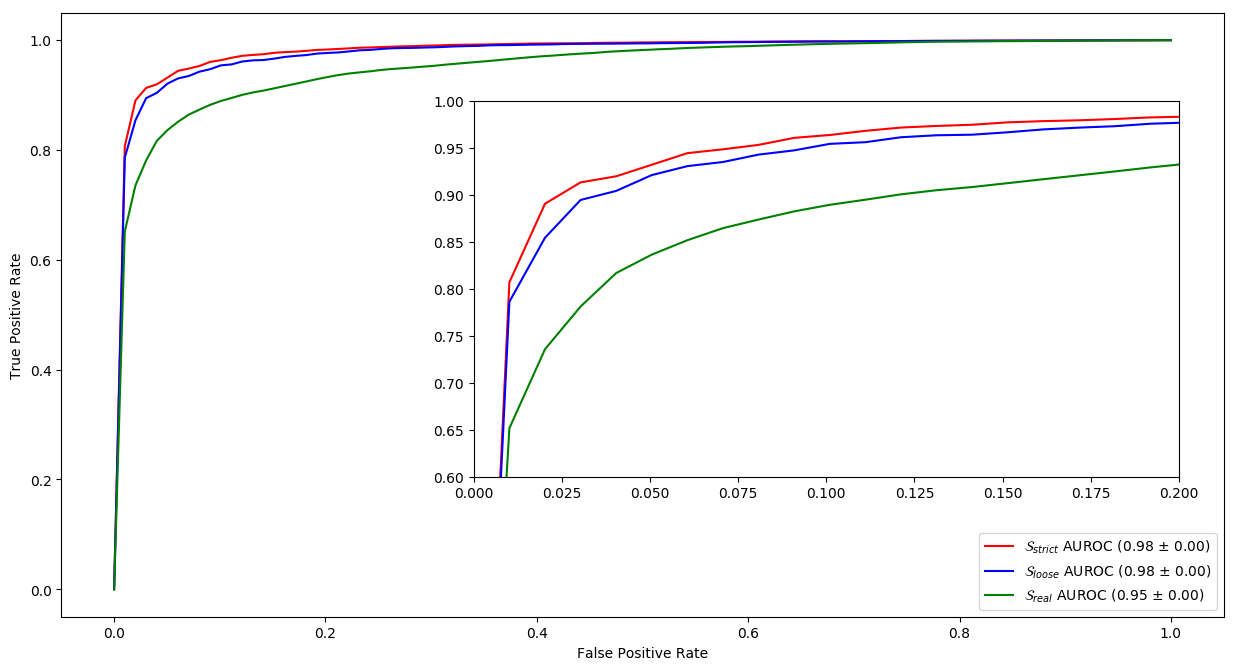
\includegraphics[width=\columnwidth]{xval_improved}
	\caption{Multi layer results for dynamic features in laboratory conditions.}
	\label{fig:improved_xval}
\end{figure}

% Adicionar seccao para resultados do multi layer apenas.

As with previous results, one notes that from $\mathcal{S}_{\strict}$ to $\mathcal{S}_{\loose}$ the results are not affected at all, when the change between the scenarios is merely in the number of malware samples.
Between $\mathcal{S}_{\loose}$ to $\mathcal{S}_{\real}$ we again note the already seen pattern, the score is lowest when using the most realistic dataset.

The comparison between scenarios does not yield any new information from what was seen in Section \ref{section:single_layer_results}.
What is more interesting is that the absolute values are boosted in all scenarios, which show indeed that using the multi-layer approach with dynamic features improve the model's results.

Having applied the same cross-validation to our modified model, obtaining interesting results, we now go over to test how our temporal based methodologies are affected.

\medskip

We start again with \textit{Past-to-Present} validation to each scenario $\mathcal{S}_{\strict}$, $\mathcal{S}_{\loose}$ and $\mathcal{S}_{\real}$.
Figure \ref{fig:pastpresent_modified} shows the \gls{auroc} at every iteration (\ie\ fold) for each scenario: 96\% for $\mathcal{S}_{\strict}$ and $\mathcal{S}_{\loose}$, and 92\% $\mathcal{S}_{\real}$.

\begin{figure}[!htb]
	\centering
	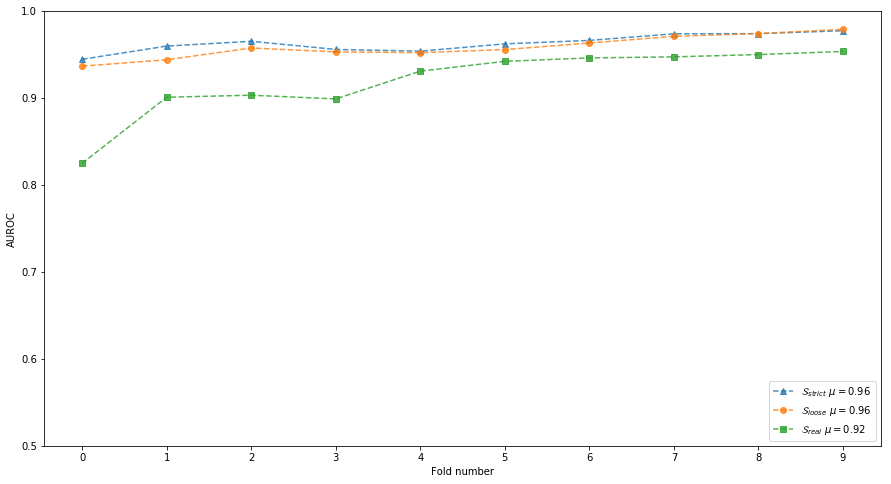
\includegraphics[width=\columnwidth]{pastpresent_improved}
	\caption[Multi layer results for dynamic features in \textit{Past-to-Present}.]{\gls{auroc} for each iteration of the \textit{Past-to-Present} evaluation. Folds order consistent with temporal order (\ie\ fold 0 contains older samples than
		fold 1)}
	\label{fig:pastpresent_modified}
\end{figure}

When comparing the average \gls{auroc} between cross-validation and \textit{Past-to-Present} validation, we note that both $\mathcal{S}_{\strict}$ and $\mathcal{S}_{\loose}$ decrease 2\%, while $\mathcal{S}_{\real}$ decreases 3\%.
This decrease is not a surprise, given the temporal consistency enforcement between samples.

The results are consistent with was previously seen in Section \ref{section:single_layer_results}, with the added factor that the absolute values are higher, and the tendency to increase is more present as we move forward in time, close to the validation set.

\medskip

Following the previous evaluation order, we now present the results using our \textit{Present-to-Past} validation methodology.
In Figure \ref{fig:presentpast_improved} we present the \gls{auroc} for each iteration, where higher folds represent older samples. Here we see values of 97\% for $\mathcal{S}_{\strict}$, 98\% for $\mathcal{S}_{\loose}$ and 96\% $\mathcal{S}_{\real}$.

\begin{figure}[!h]
	\centering
	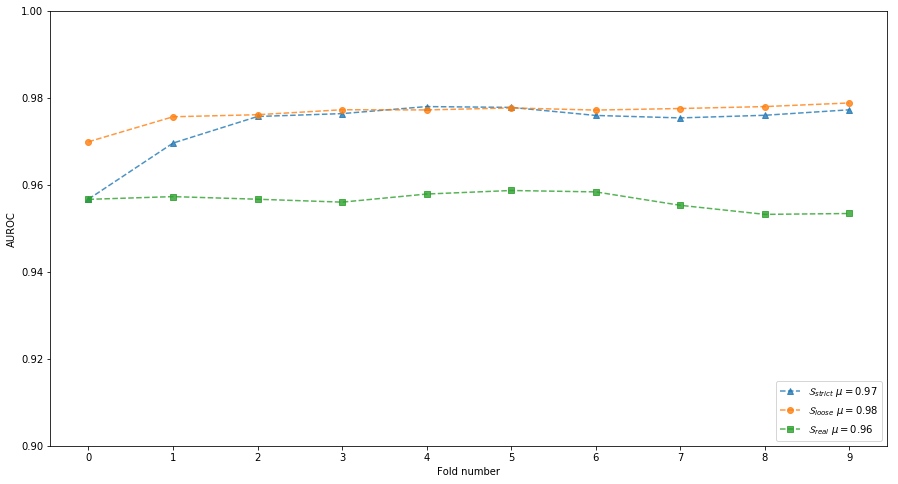
\includegraphics[width=\columnwidth]{presentpast_improved}
	\caption[Multi layer results for dynamic features in \textit{Present-to-Past}.]{\gls{auroc} for each iteration of the \textit{Present-to-Past} evaluation. Folds order is the inverse of temporal order (\ie\ fold 0 contains newer samples than fold 1)}
	\label{fig:presentpast_improved}
\end{figure}

When comparing to cross-validation, we note $\mathcal{S}_{\strict}$ is affected as expected, whereas $\mathcal{S}_{\loose}$ is not.
The fact that the datasets vary in size and so the amount of goodware and malware used for testing in each may vary, can justify how the $\mathcal{S}_{\loose}$ is not affected, whereas $\mathcal{S}_{\strict}$ is.

$\mathcal{S}_{\real}$ seems to have a higher value than in cross-validation, but it is rounded, which slightly inflates the value.
In practice both cross-validation and \textit{Present-to-Past} are identical for $\mathcal{S}_{\real}$.

In these results, the noticeable increase in the first 3 folds (0, 1 and 2) for $\mathcal{S}_{\strict}$ and $\mathcal{S}_{\loose}$ goes even more in favor with our argument that samples closer to the validation set benefit the model.
More so as the \gls{auroc} stabilizes from those folds on.
This effect is not as accentuated for $\mathcal{S}_{\real}$, although using more and older folds do not provide significantly better results.

\medskip

Finally, we retest how a reduced training set behaves in our scenarios by using our \textit{Temporal Window} methodology.
As previously mentioned, the first 3 folds seem to provide enough information to obtain good results, hence we apply the same sliding window size of $n=3$ as in Section \ref{section:single_layer_results}.
Starting at the oldest fold, we apply this window and slide it by one fold at each iteration.
Figure \ref{fig:slidingwindow_modified} shows how all our scenarios $\mathcal{S}_{\strict}$, $\mathcal{S}_{\loose}$ and $\mathcal{S}_{\real}$ score the same \gls{auroc} of 94\%, although with different curves.

For $\mathcal{S}_{\strict}$, $\mathcal{S}_{\loose}$ the score is equally and negatively affected by 4\%.
The jagged curve on both scenarios indicate that slight changes on the \gls{fpr} threshold have significant impact on the \gls{tpr}, this may be caused by the smaller dataset size, which in turn creates uneven folds for malware and goodware.

\begin{figure}[!h]
	\centering
	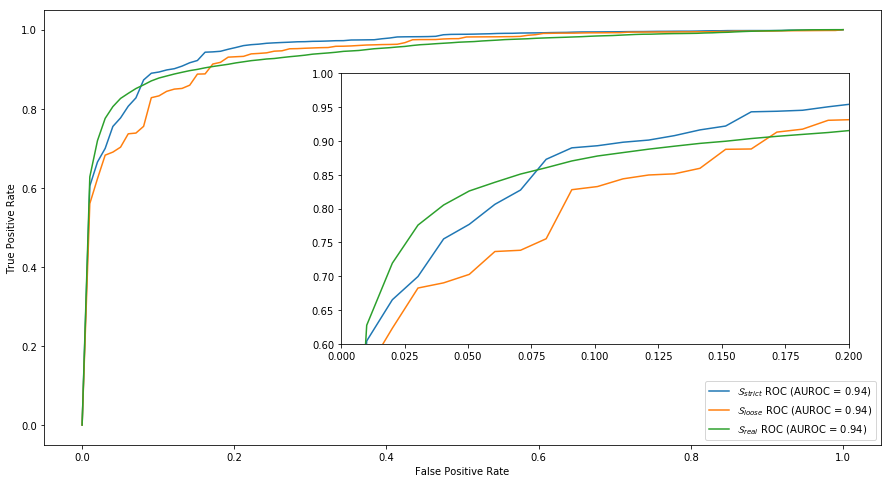
\includegraphics[width=\columnwidth]{Figures/slidingwindow_improved.png}
	\caption[Multi layer results for dynamic features in \textit{Temporal Window}.]{\gls{auroc} for our three scenarios, under the \textit{Temporal Window} methodology.}
	\label{fig:slidingwindow_modified}
\end{figure}

For $\mathcal{S}_{\real}$, the fact that it only loses 1\% when compared to cross-validation shows that indeed our argument about reducing the training set size is sustained.
Its curve is much smoother when compared to the previous scenarios, as the dataset is bigger and more even.

\medskip

%As a closing remark, we reaffirm on how it is possible to yield reasonable results when considering temporal consistent samples, specifically in this improved model, which not only uses more features, but has the ability to provide more information regarding a malware sample, as it can discriminate malware classes due to its multi layer design.
The improved layer results are summarized in Table \ref{tab:multilayer_results}.

\begin{table}[!htb]
	\renewcommand{\arraystretch}{1.2} % more space between rows
	\centering
	\begin{tabular}{ccccc}
		AUROC & $\DS_\strict$ & $\DS_\loose$ & $\DS_\real$ & Train/Test \%\\
		\hline
		Cross-Validation & 0.98 & 0.98 & 0.95 & 90 / 10\\
		Past-to-Present & 0.96 & 0.96 & 0.92 & 10 to 90 / 10\\
		Present-to-Past & 0.97 & 0.98 & 0.96 & 10 to 90 / 10\\
		Sliding-Window & 0.94 & 0.94 & 0.94 & 30 / 10\\
		\hline
	\end{tabular}
	\medskip
	\caption{Multi layer results summary.}
	\label{tab:multilayer_results}
\end{table}

%!TEX root = main.tex

\section{Discussion}\label{sec:discussion}

We have proposed different scenarios, based on different labeling metrics, to study laboratory \textit{vs} real-world conditions. Our scenarios, $\mathcal{S}_{\strict}$, $\mathcal{S}_{\loose}$ and $\mathcal{S}_{\real}$, vary both in reliability and size, going from a more reliable and small dataset to a larger and less reliable one.
This (un)reliability is due to the fact that for real world samples there is usually no agreement among vendors on how to classify a given sample, and for that we had to assign a labeling to such samples according to our proposed metrics.
We have developed several comparative analysis between these three scenarios, to evaluate how much the nature of the dataset can influence the results.
We have split the analysis into two major validation conditions: the cross validation methodology, where the time consistency is discarded; and temporal-based methodologies.
We tested our methodologies by using a simple \gls{lr} model, which was then improved to transmit better information and to use more features.

Following a cross-validation methodology, we have confirmed our intuitions: $\mathcal{S}_{\strict}$ showed up an \gls{auroc} of 0.91, $\mathcal{S}_{\loose}$ have presented 0.9, whereas $\mathcal{S}_{\real}$ decreased to 0.75. 
As we have argued, the results on $\mathcal{S}_{\strict}$ are justified by factors like a small and reliable dataset, and the use of cross-validation, which mixes samples and ignores possible dependencies between them.
This scenario is composed by very well-known and analyzed samples.
Although $\mathcal{S}_{\loose}$ slightly relaxes these requirements, it is still composed by very well-known samples, which partially justifies the comparable \gls{auroc} (0.90).
But this difference is interesting, as although the number of malware labeled samples increased significantly, the results are not that affected.
As we have noticed, this might also suggest that vendors do converge on their definition of malware, under our $\mathcal{M}_{\loose}$ metric. 
The changes observed from $\mathcal{S}_{\loose}$ to $\mathcal{S}_{\real}$ are more remarkable, but somehow expected.
The metric that labels malware and goodware for the scenario $\mathcal{S}_{\real}$ disregards the cross-check from outside repositories, which in turn degrades the reliability significantly, while increasing the dataset size notably. 
As we have already noticed, we attribute the result's degradation mainly to the unreliability of goodware labeling, not only because we have previously seen that the increase in malware does not significantly impact the results (from $\SS_\strict$ to $\SS_\loose$), but also due to the tendency for false negatives in vendors (Figure~\ref{fig:distribution_changes}), which in turn lead us to incorrectly label as goodware some of the malicious samples in $\DD$.

When temporal consistency comes into play, the results on different scenarios do not differ much, nevertheless we can observe more pronounce trends.
The great conclusion that we can take stands on the relative position of the training set with respect to the validation set and its size.
Indeed, samples closer to the validation set seem to benefit the model.
We argue that there should be an ideal number of necessary training folds (30\% of the dataset), temporally consistent with the validation fold (10\% of the dataset), needed to maximize the overall score.
This supports our argument that we can reduce the size of the training set, without losing any significant score.

We finished our analysis by validating this temporal-based results.
For this purpose, we have defined a sliding window for each scenario, with the above parameters, that moved forward in time (1 fold at a time) and obtained the \gls{auroc} values of 0.89 for $\mathcal{S}_{\strict}$, 0.88 for $\mathcal{S}_{\loose}$ and 0.73 for $\mathcal{S}_{\real}$.
Comparing these results with the baseline cross-validation, we note a very slight decrease for each scenario.
This decrease, although not significant, was more than expected due to the enforcement of temporal consistency as well as the significant reduction of the size of the training set. 
We should highlight that these results should be much closer to reality than the ones provided by cross validation techniques, since we are requiring temporal consistency and also a reasonable amount of data for training purposes, which might be a relevant issue in a few year's time.
Indeed, aiming at complementing antivirus' vendors techniques with machine learning, we should not expect to gather and use all the samples ever seen for training purposes, and these results may be very useful on the choice of the right training set.

Finally, we describe multiple improvements to our base model $\LR$ in order to improve the overall results.
We started by using a multi layer approach to build a new model $\mathcal{E}$, which enables the extraction of more detailed information regarding a malicious sample, specifically the malware class it belongs.
We also introduced three new dynamic features, to improve the amount of information obtained from the samples.
After applying the same evaluation methodologies to our new model $\mathcal{E}$, we observed an increase in all cases.
We note that the bigger the dataset, the higher the improvement, as $\mathcal{S}_{\strict}$ increased by 0.07 (cross-validation), $\mathcal{S}_{\loose}$ by 0.08 and $\mathcal{S}_{\real}$ (cross-validation) by 0.27 (\textit{present-to-past}).
This comes to show how the model was better able to learn from the new features.

%!TEX root = main.tex

\section{Conclusion}\label{sec:conclusion}

In this paper we analyzed how \gls{ml} techniques fit into the scope of malware detection and how could the chosen dataset influence the results of the classifier. 

Given the non-existence of a common agreement on how to label samples in a real world dataset, we have proposed three different metrics for labeling these samples, and presented three different scenarios, ranging from a more simulated scenario, where better results are achieved, to more realistic ones, where the \gls{auroc} results can go down by 23\%.
We have analyzed the different scenarios mainly on two kind of conditions: the laboratory conditions where the standard cross-validation methodology was applied discarding the importance of \emph{time} in malware detection, and temporal-consistent techniques where we have trained and validated the model in a temporal-consistent manner.
We have shown that for a modest compromise in accuracy temporal-consistent methodologies are adequate to classify malware samples.

We have also concluded that we can reduce the size of the training dataset to avoid the need of training with all ever seen samples, and argue on how much it can be reduced without compromising optimal results.

Having a sound understanding of the effects of different methodologies, we improved our model to yield higher results.

We believe that the pertinent question of how much should we seek for great results on \gls{ml} techniques applied to malware detection is worth to be further discussed, bearing in mind that it leads to classifiers that would not perform better over realistic conditions. 
As future work we aim at optimizing our logistic regression model, at increasing and optimizing the features, and finally, at developing a supervised learning methodology to classify malware samples according to the main malware families.



\bibliographystyle{IEEEtran}
\bibliography{IEEEabrv,articlebib}
%
% \newpage
% \appendix
% %!TEX root = main.tex
\color{red}

\begin{figure}[h!]
	\centering
	\includegraphics[width=\columnwidth]{roc_tc_strict_1}
	\caption{\gls{roc} and \gls{auroc} for $\mathcal{S}_{strict}$ under \textit{Past-to-Present} .}
	\label{fig:roc_tc_strict_1}
\end{figure}

\begin{figure}[h!]
	\centering
	\includegraphics[width=\columnwidth]{roc_tc_loose_1}
	\caption{\gls{roc} and \gls{auroc} for $\mathcal{S}_{loose}$ under \textit{Past-to-Present} .}
	\label{fig:roc_tc_loose_1}
\end{figure}

\begin{figure}[h!]
	\centering
	\includegraphics[width=\columnwidth]{roc_tc_real_1}
	\caption{\gls{roc} and \gls{auroc} for $\mathcal{S}_{real}$ under \textit{Past-to-Present} .}
	\label{fig:roc_tc_real_1}
\end{figure}

\begin{figure}[h!]
	\centering
	\includegraphics[width=\columnwidth]{roc_tc_strict_2}
	\caption{\gls{roc} and \gls{auroc} for $\mathcal{S}_{strict}$ under \textit{Present-to-Past} .}
	\label{fig:roc_tc_strict_2}
\end{figure}

\begin{figure}[h!]
	\centering
	\includegraphics[width=\columnwidth]{roc_tc_loose_2}
	\caption{\gls{roc} and \gls{auroc} for $\mathcal{S}_{loose}$ under \textit{Present-to-Past} .}
	\label{fig:roc_tc_loose_2}
\end{figure}

\begin{figure}[h!]
	\centering
	\includegraphics[width=\columnwidth]{roc_tc_real_2}
	\caption{\gls{roc} and \gls{auroc} for $\mathcal{S}_{real}$ under \textit{Present-to-Past} .}
	\label{fig:roc_tc_real_2}
\end{figure}


\end{document}
